\documentclass[12pt,a4paper]{report}

% Importation des packages
% Encodage et langue
\usepackage[utf8]{inputenc}
\usepackage[T1]{fontenc}
\usepackage[french]{babel}

% Mise en page
\usepackage[a4paper,margin=2.5cm,top=3cm,bottom=3cm]{geometry}
\usepackage{setspace}
\onehalfspacing

% Graphiques et images
\usepackage{graphicx}
\usepackage{float}
\usepackage{caption}
\usepackage{subcaption}

% Tableaux
\usepackage{booktabs}
\usepackage{array}
\usepackage{longtable}
\usepackage{multirow}

% Mathématiques
\usepackage{amsmath}
\usepackage{amssymb}

% Listings et code
\usepackage{listings}
\usepackage{xcolor}

% Liens et navigation
\usepackage{hyperref}
\usepackage{titlesec}

% En-têtes et pieds de page
\usepackage{fancyhdr}

% Table des matières
\usepackage{tocloft}
\usepackage{tocbibind}

% Listes
\usepackage{enumitem}

% Configuration des listings pour le code
\lstset{
    basicstyle=\ttfamily\footnotesize,
    keywordstyle=\color{blue}\bfseries,
    commentstyle=\color{green!60!black},
    stringstyle=\color{red},
    breaklines=true,
    frame=single,
    numbers=left,
    numberstyle=\tiny\color{gray},
    tabsize=2,
    showstringspaces=false
}


% Configuration du document
% Configuration des en-têtes et pieds de page
\pagestyle{fancy}
\fancyhf{}
\fancyhead[L]{\leftmark}
\fancyhead[R]{\thepage}
\fancyfoot[C]{Rapport de Stage - PICU}

% Configuration des titres de chapitres
\titleformat{\chapter}[display]
{\normalfont\huge\bfseries\centering}{\chaptertitlename\ \thechapter}{20pt}{\Huge}

% Profondeur de la table des matières (chapitres + sections principales uniquement)
\setcounter{tocdepth}{1}
\setcounter{secnumdepth}{3}

% Configuration de la table des matières
\setlength{\cftbeforechapskip}{10pt}
\setlength{\cftbeforesecskip}{4pt}
\setlength{\cftchapindent}{0pt}
\setlength{\cftsecindent}{1.5em}

% Configuration des liens hypertexte
\hypersetup{
    colorlinks=true,
    linkcolor=blue,
    filecolor=magenta,
    urlcolor=cyan,
    citecolor=blue
}

% Configuration des listes
\setlist[itemize]{itemsep=5pt}
\setlist[enumerate]{itemsep=5pt}

% Configuration des légendes
\captionsetup[figure]{labelfont=bf,textfont=normal}
\captionsetup[table]{labelfont=bf,textfont=normal}

% Configuration des marges pour les listings
\lstset{
    frame=single,
    frameround=tttt,
    rulecolor=\color{black!30}
}

% Inclusion d'image tolerante : essaie .png, .jpg puis .jpeg.
% Usage : \IncludeImg[largeur]{nom_sans_extension}
% Exemple : \IncludeImg[4cm]{logo_upf}  -> images/logo_upf.png (ou .jpg/.jpeg)
\newcommand{\IncludeImg}[2][\linewidth]{%
    \IfFileExists{images/#2.png}{\includegraphics[width=#1]{images/#2.png}}{%
    \IfFileExists{images/#2.jpg}{\includegraphics[width=#1]{images/#2.jpg}}{%
    \IfFileExists{images/#2.jpeg}{\includegraphics[width=#1]{images/#2.jpeg}}{%
    \IfFileExists{images/#2.PNG}{\includegraphics[width=#1]{images/#2.PNG}}{%
    \IfFileExists{images/#2.JPG}{\includegraphics[width=#1]{images/#2.JPG}}{%
        \fbox{\parbox{#1}{\centering\vspace{1cm}À insérer : \texttt{images/#2.png}\vspace{1cm}}}}%
    }}}}}%


\begin{document}

% Page de garde
\begin{titlepage}
    \centering
    \vspace*{\fill}

    % Logo de l'université → déposer : images/logo_upf.png (ou .jpg/.jpeg)
    \IncludeImg[3cm]{logo_upf}

    {\Large\textbf{Université Privée de Fès}}\\[0.3cm]
    {\large Département Informatique}\\[0.9cm]

    % Logo du CHU → déposer : images/logo_chu.png (ou .jpg/.jpeg)
    \IncludeImg[3cm]{logo_chu}

    {\Large\textbf{Centre Hospitalier Universitaire Hassan II de Fès}}\\[0.8cm]

    \rule{12cm}{0.4pt}\\[0.8cm]

    {\Huge\textbf{Rapport de Stage de Fin d'Année}}\\[0.5cm]
    {\Large PICU}\\[0.3cm]
    {\large Plateforme Intelligente de Coordination des Urgences}\\[0.8cm]

    \rule{12cm}{0.4pt}\\[0.8cm]

    {\Large\textbf{Présenté par :}}\\[0.3cm]
    {\Large Younes Basir}\\[0.7cm]

    {\Large\textbf{Année Universitaire :}}\\[0.3cm]
    {\Large 2024-2025}

    \vspace*{\fill}
\end{titlepage}


% Remerciements
\chapter*{Remerciements}
\addcontentsline{toc}{chapter}{Remerciements}

Je tiens à exprimer ma profonde gratitude envers toutes les personnes qui ont contribué, de près ou de loin, à la réussite de ce stage et à l'élaboration de ce rapport.

Je remercie tout d'abord mon encadrant de stage au sein du Centre Hospitalier Universitaire Hassan II de Fès, pour sa disponibilité, ses conseils précieux et son accompagnement tout au long de cette période. Sa confiance et son expertise m'ont permis de mener à bien ce projet dans les meilleures conditions.

Je tiens également à remercier l'ensemble du personnel du département informatique du CHU Hassan II pour leur accueil chaleureux et leur collaboration. Leur professionnalisme et leur volonté de partager leurs connaissances ont grandement enrichi mon expérience.

Mes remerciements vont également à mes professeurs de l'Université Privée de Fès, notamment ceux du département informatique, pour la qualité de l'enseignement reçu et la préparation rigoureuse qui m'a permis d'acquérir les compétences nécessaires à la réalisation de ce projet.

Je remercie également l'ensemble de l'équipe pédagogique de l'UPF pour leur suivi et leur soutien tout au long de mon parcours universitaire.

Enfin, je remercie ma famille pour son soutien inconditionnel, sa patience et son encouragement constants tout au long de mes études et particulièrement durant la réalisation de ce stage.


% Résumé et Abstract
\chapter*{Résumé}
\addcontentsline{toc}{chapter}{Résumé}

Ce rapport de stage présente la conception, la réalisation et l'évaluation de PICU (Plateforme Intelligente de Coordination des Urgences), une application web destinée au service des urgences du Centre Hospitalier Universitaire Hassan II de Fès. Le projet répond à un double constat : la dispersion de l'information entre les acteurs (accueil, triage, médecine) et l'absence de visibilité en temps réel sur l'occupation des zones, des salles et des lits.

Plutôt que de décrire uniquement des fonctionnalités, ce rapport met l'accent sur la \textbf{démarche d'ingénierie logicielle} : analyse des besoins, méthodologie de développement, modélisation, conception de la base de données, architecture, assurance qualité, sécurité et industrialisation. L'originalité du travail réside dans la transformation d'un processus hospitalier informel en un \textbf{workflow transactionnel} explicite : une machine à états de la visite (\texttt{waiting}, \texttt{placed}, \texttt{in\_treatment}, puis états terminaux), des transitions autorisées, des priorités cliniques P1--P5, des files d'attente calculées et une gestion des ressources verrouillée en base de données.

La plateforme est construite sur une architecture client-serveur : un frontend React~19 / Vite / TailwindCSS, un backend Node.js / Express exposant une API REST, une base PostgreSQL (hébergée sur Neon) et une communication temps réel par \textbf{Socket.IO}. La sécurité repose sur un contrôle d'accès par rôle et capacités (RBAC), des jetons JWT, des transactions PostgreSQL et une piste d'audit exhaustive (\texttt{visit\_events}). Des modules avancés complètent le socle : supervision opérationnelle avec indicateurs SLA, gestion du cycle de vie des lits, demandes de transfert et de relève, examens et tâches de soin, suivi analytique, ainsi qu'une couche d'\textbf{assistance IA} fondée sur NVIDIA NIM (triage, flux de lits, capacité, documentation) fonctionnant en mode supervisé avec approbation humaine.

La qualité est vérifiée par une stratégie de tests explicite : tests unitaires et d'intégrité basés sur \texttt{node:test} (invariants de ressources, règles de supervision, intelligence d'enregistrement, analytics), tests fonctionnels par rôle, tests de concurrence sur l'affectation des lits et scénario de bout en bout. L'industrialisation s'appuie sur Git, des hooks pre-commit et un pipeline GitHub Actions « secret guard ».

Ce rapport est organisé en six chapitres. Le premier présente l'organisme d'accueil et le contexte du projet. Le deuxième formalise l'analyse et la spécification des besoins. Le troisième expose la méthodologie et la conception. Le quatrième détaille la réalisation. Le cinquième traite de l'assurance qualité, de la sécurité et de la CI/CD. Le sixième dresse l'évaluation, le bilan et les perspectives, notamment l'assistance IA NVIDIA NIM.

\textbf{Mots-clés :} PICU, Urgences, Workflow transactionnel, Machine à états, Triage IA, RBAC, PostgreSQL, Socket.IO, CI/CD, Qualité logicielle

\chapter*{Abstract}
\addcontentsline{toc}{chapter}{Abstract}

This internship report presents the design, implementation and evaluation of PICU (Intelligent Emergency Coordination Platform), a web application for the emergency department of the Hassan II University Hospital in Fez. The project addresses two problems: information dispersion between actors (registration, triage, physicians) and the lack of real-time visibility over zone, room and bed occupancy.

Rather than describing features only, this report emphasizes the \textbf{software engineering process}: requirements analysis, development methodology, modelling, database design, architecture, quality assurance, security and deployment automation. The core contribution is the transformation of an informal hospital process into an explicit \textbf{transactional workflow}: a visit state machine (\texttt{waiting}, \texttt{placed}, \texttt{in\_treatment}, then terminal states), allowed transitions, P1--P5 clinical priorities, computed waiting lists and database-locked resource management.

The platform uses a client-server architecture: a React~19 / Vite / TailwindCSS frontend, a Node.js / Express REST API, a PostgreSQL database (hosted on Neon) and \textbf{Socket.IO} real-time communication. Security relies on role and capability-based access control (RBAC), JWT tokens, PostgreSQL transactions and a complete audit trail (\texttt{visit\_events}). Advanced modules complete the foundation: supervision with SLA indicators, bed lifecycle management, transfer and handoff requests, exams and care tasks, analytics, and an \textbf{AI assistance} layer built on NVIDIA NIM (triage, bed flow, capacity, documentation) operating under human supervision.

Quality is verified through an explicit testing strategy: unit and integrity tests based on \texttt{node:test}, role-based functional tests, concurrency tests on bed assignment, and an end-to-end scenario. Delivery automation relies on Git, pre-commit hooks and a GitHub Actions “secret guard” pipeline.

The report is organised into six chapters: host organization and context; requirements analysis; methodology and design; implementation; quality assurance, security and CI/CD; and evaluation, review and perspectives.

\textbf{Keywords:} PICU, Emergency Department, Transactional Workflow, State Machine, AI Triage, RBAC, PostgreSQL, Socket.IO, CI/CD, Software Quality


% Table des matières
\tableofcontents
\cleardoublepage

% Liste des figures
\listoffigures
\cleardoublepage

% Liste des tableaux
\listoftables
\cleardoublepage

% Liste des acronymes
\chapter*{Liste des acronymes}
\addcontentsline{toc}{chapter}{Liste des acronymes}

\begin{tabular}{ll}
\textbf{API} & Application Programming Interface \\
\textbf{BNF} & Besoin Non Fonctionnel \\
\textbf{CHU} & Centre Hospitalier Universitaire \\
\textbf{CI/CD} & Intégration Continue / Livraison Continue \\
\textbf{CRUD} & Create, Read, Update, Delete \\
\textbf{FHIR} & Fast Healthcare Interoperability Resources \\
\textbf{HL7} & Health Level Seven \\
\textbf{IA} & Intelligence Artificielle \\
\textbf{JSON} & JavaScript Object Notation \\
\textbf{JSONB} & Type JSON binaire de PostgreSQL \\
\textbf{JWT} & JSON Web Token \\
\textbf{KPI} & Key Performance Indicator \\
\textbf{LLM} & Large Language Model \\
\textbf{NIM} & NVIDIA Inference Microservices \\
\textbf{PICU} & Plateforme Intelligente de Coordination des Urgences \\
\textbf{RAG} & Retrieval-Augmented Generation \\
\textbf{RBAC} & Role-Based Access Control \\
\textbf{REST} & Representational State Transfer \\
\textbf{SIH} & Système d'Information Hospitalier \\
\textbf{SLA} & Service Level Agreement \\
\textbf{UML} & Unified Modeling Language \\
\end{tabular}

\cleardoublepage

% Introduction générale
\chapter*{Introduction générale}
\addcontentsline{toc}{chapter}{Introduction générale}

\section{Contexte général}

Les services des urgences hospitaliers constituent un maillon critique du système de santé : ils assurent la prise en charge immédiate de patients dont l'état peut s'aggraver en quelques minutes. Le Centre Hospitalier Universitaire Hassan II de Fès, établissement de référence régional, accueille en permanence un flux important de patients adultes et pédiatriques. La qualité de cet accueil dépend d'une coordination rigoureuse entre l'accueil administratif, le triage clinique, l'orientation vers les zones spécialisées et la disponibilité des ressources (salles, lits, personnel).

Or, dans de nombreux services, cette coordination reste largement manuelle : transmissions orales, supports papier et outils non intégrés. Il en résulte des pertes d'information, des délais de prise en charge difficiles à mesurer et une visibilité limitée sur l'occupation réelle des zones.

\section{Problématique}

La problématique centrale de ce stage peut être formulée ainsi :

\begin{quote}
\textit{Comment concevoir et réaliser une plateforme numérique capable de formaliser le workflow des urgences, de garantir la cohérence et la traçabilité du parcours patient de l'arrivée à la sortie, d'offrir une vision temps réel partagée entre les rôles, tout en intégrant une assistance IA sous contrôle humain ?}
\end{quote}

Cette problématique recouvre trois difficultés techniques : l'absence d'un modèle d'état explicite du parcours patient ; la gestion concurrente des ressources partagées (deux infirmiers ne doivent jamais affecter le même lit) ; et la définition d'une frontière stricte entre les décisions automatisables et les décisions strictement cliniques.

\section{Objectifs du projet}

Le projet PICU (Plateforme Intelligente de Coordination des Urgences) poursuit les objectifs suivants :

\begin{itemize}
    \item \textbf{formaliser} le parcours patient en une machine à états transactionnelle, source de vérité unique ;
    \item \textbf{centraliser} la gestion des patients, des visites, des ressources et des équipes de salle ;
    \item \textbf{offrir} une vision en temps réel de l'activité, diffusée par Socket.IO à tous les postes ;
    \item \textbf{garantir} l'intégrité et la traçabilité de chaque décision (\texttt{visit\_events}) ;
    \item \textbf{assurer} la sécurité par un contrôle d'accès par rôle et capacités (RBAC) et des jetons JWT ;
    \item \textbf{assister} les équipes par une couche IA (triage, lits, capacité, documentation) strictement supervisée ;
    \item \textbf{industrialiser} le cycle de vie du code (versioning, hooks, intégration continue).
\end{itemize}

\section{Démarche d'ingénierie adoptée}

Le rapport met délibérément l'accent sur la démarche d'ingénierie plutôt que sur une simple énumération de fonctionnalités. Pour chaque décision majeure, nous nous efforçons de présenter le problème initial, les solutions envisagées, la solution retenue, sa justification technique et la manière dont son bon fonctionnement a été vérifié. Le projet a été mené de façon itérative, organisé autour de jalons versionnés : socle transactionnel, enrichissement du parcours (V3), supervision et ressources (V4), puis couche d'assistance IA.

\section{Méthodologie et outils}

La méthodologie combine une approche incrémentale, une modélisation UML en amont (cas d'utilisation, états, séquence, classes), une conception de base de données normalisée et un cycle qualité continu. Les principaux outils sont :

\begin{itemize}
    \item \textbf{Git} pour la gestion de versions, avec une convention de commits et des hooks \texttt{pre-commit} ;
    \item \textbf{GitHub Actions} pour les vérifications automatiques (pipeline « secret guard ») ;
    \item \textbf{Node.js} et le lanceur de tests natif \texttt{node:test} pour l'exécution automatisée ;
    \item \textbf{Draw.io / Mermaid} pour les diagrammes UML ;
    \item \textbf{Neon} comme hébergement PostgreSQL managé.
\end{itemize}

\section{Organisation du rapport}

Le rapport est structuré en six chapitres :

\begin{itemize}
    \item \textbf{Chapitre 1} : Organisme d'accueil et contexte du projet ;
    \item \textbf{Chapitre 2} : Analyse et spécification des besoins ;
    \item \textbf{Chapitre 3} : Méthodologie et conception du système ;
    \item \textbf{Chapitre 4} : Réalisation de la plateforme PICU ;
    \item \textbf{Chapitre 5} : Assurance qualité, sécurité et CI/CD ;
    \item \textbf{Chapitre 6} : Évaluation, bilan et perspectives.
\end{itemize}

Le document se termine par une conclusion générale, une bibliographie, une webographie et des annexes.


% Chapitre 1 : Organisme d'accueil et contexte du projet
\chapter{Organisme d'accueil et contexte du projet}

\section{Introduction}

Ce chapitre présente l'organisme d'accueil, le cadre du stage, le fonctionnement actuel du service des urgences, les limites identifiées et la solution proposée. Il pose ainsi le \textit{pourquoi} du projet avant d'aborder le \textit{comment} dans les chapitres suivants.

\section{Présentation de l'organisme d'accueil}

\subsection{Le CHU Hassan II de Fès}

Le Centre Hospitalier Universitaire Hassan II de Fès est un établissement public de santé de référence pour la région Fès--Meknès. Il assure trois missions indissociables :

\begin{itemize}
    \item \textbf{Soins} : prise en charge des urgences vitales et non vitales, hospitalisation et spécialités ;
    \item \textbf{Enseignement} : formation des étudiants en médecine, des internes et du personnel paramédical ;
    \item \textbf{Recherche} : développement de projets innovants, dont l'informatisation des services cliniques.
\end{itemize}

\subsection{Le service des urgences}

Le service des urgences fonctionne 24~heures sur~24 et reçoit des patients adultes et pédiatriques. Il est organisé en zones spécialisées~: Triage, Déchocage, Pédiatrie, Médecine, Chirurgie et Observation. Chaque zone regroupe des salles, des lits et un personnel affecté selon la charge. Le Déchocage et la zone critique prennent en charge les urgences vitales, tandis que les zones Médecine et Chirurgie absorbent la majorité du flux.

\subsection{Le Département Informatique}

Le stage s'est déroulé au sein du Département Informatique de l'établissement, en lien fonctionnel avec l'encadrement médical du service des urgences. Ce positionnement a permis de confronter en continu les choix techniques aux contraintes cliniques et organisationnelles réelles.

\section{Cadre du stage}

\subsection{Objet et périmètre}

L'objet du stage est la conception et la réalisation d'une plateforme de coordination des urgences, PICU, couvrant le parcours du patient depuis son enregistrement à l'accueil jusqu'à la clôture de sa prise en charge. Le périmètre fonctionnel comprend l'accueil, le triage, la file d'attente, l'orientation et le placement, la prise en charge médicale, la gestion des ressources et la supervision.

\subsection{Livrables attendus}

\begin{itemize}
    \item une application web fonctionnelle (frontend, backend, base de données) ;
    \item un modèle de données et une documentation d'architecture ;
    \item une stratégie de tests et des résultats de validation ;
    \item le présent rapport de stage et un support de soutenance.
\end{itemize}

\section{Fonctionnement actuel du service des urgences}

\subsection{Accueil et enregistrement}

Le réceptionniste recueille l'identité du patient, le motif de consultation et le mode d'arrivée. Un dossier administratif est créé ou mis à jour. Dans le fonctionnement manuel, cette étape repose sur des saisies répétées et des supports hétérogènes.

\subsection{Triage clinique}

Une infirmière trieuse évalue la gravité et attribue une priorité, généralement de P1 (urgent vital) à P5 (non urgent). Le triage est une décision clinique qui conditionne l'ordre de prise en charge.

\subsection{Orientation et prise en charge}

Après triage, le patient est orienté vers une zone, appelé depuis la file d'attente, placé sur une ressource (lit, fauteuil, box) puis pris en charge par un médecin. En cas d'erreur d'orientation, le médecin doit pouvoir transférer le patient vers une autre spécialité.

\subsection{Gestion de la file d'attente et des ressources}

La file est organisée par priorité clinique puis par ordre d'arrivée. La disponibilité des lits et la charge des salles déterminent la fluidité du service.

\section{Limites du fonctionnement actuel}

L'étude de l'existant met en évidence plusieurs limites :

\begin{itemize}
    \item \textbf{absence de visibilité temps réel} sur l'occupation des zones et des lits ;
    \item \textbf{coordination difficile} entre accueil, soins et médecine, faute d'un référentiel commun ;
    \item \textbf{ressaisies et pertes d'information}, sans traçabilité fiable des décisions ;
    \item \textbf{risque de conflits d'affectation} lorsque plusieurs soignants manipulent les mêmes ressources ;
    \item \textbf{difficulté à mesurer la performance} (temps d'attente, goulots d'étranglement, qualité du triage).
\end{itemize}

Ces limites justifient une refonte numérique dont le cœur n'est pas un écran supplémentaire, mais un \textbf{modèle de processus explicite et transactionnel}.

\section{Problématique et solution proposée}

\subsection{Problématique}

Telle que formulée en introduction, la problématique interroge la capacité à formaliser le parcours patient, à garantir sa cohérence concurrente et à offrir une vision partagée en y intégrant une assistance IA supervisée.

\subsection{Solution proposée}

PICU est une application web centralisée offrant :

\begin{itemize}
    \item des \textbf{tableaux de bord par rôle} (accueil, infirmier, médecin, chef de service, administrateur) ;
    \item un \textbf{moteur de workflow transactionnel} où chaque action de visite est atomique et auditable ;
    \item une \textbf{gestion unifiée} des patients, des visites, des ressources et des équipes de salle ;
    \item une \textbf{communication temps réel} par Socket.IO synchronisant tous les postes ;
    \item une \textbf{couche de supervision} (SLA, alertes, blocages) pour le chef de service ;
    \item une \textbf{assistance IA} optionnelle et supervisée (triage, lits, capacité, documentation).
\end{itemize}

\subsection{Apports attendus}

La valeur attendue est triple : \textit{organisationnelle} (réduction des délais et de la charge cognitive), \textit{qualité} (traçabilité et fiabilité des données) et \textit{décisionnelle} (indicateurs objectifs pour piloter le service).

\section{Distinction entre prototype et système validé}

Il importe de préciser le statut du livrable. PICU est une \textbf{plateforme développée et évaluée dans le cadre du stage}. Elle n'est pas déployée en production clinique et n'a pas fait l'objet d'une validation médicale officielle par l'établissement. Les fonctionnalités et les modules d'IA y sont donc présentés \textbf{selon leur état réel d'implémentation} : socle transactionnel mature, modules V3/V4 opérationnels en environnement de démonstration, et assistance IA disponible mais en mode supervisé, non autonome en production. Cette honnêteté de cadrage est une exigence d'ingénierie pour une application de santé.

\section{Conclusion}

Ce chapitre a présenté l'organisme d'accueil, le fonctionnement des urgences, ses limites et la solution PICU, en insistant sur la nécessité d'un workflow explicite et traçable. Le chapitre suivant formalise l'analyse et la spécification des besoins.


% Chapitre 2 : Analyse et spécification des besoins
\chapter{Analyse et spécification des besoins}

\section{Introduction}

Ce chapitre transforme les constats du chapitre précédent en exigences exploitables. Il identifie les acteurs, distingue les besoins fonctionnels et non fonctionnels, formalise les \textbf{règles métier} structurantes, présente les cas d'utilisation puis la traçabilité entre exigences, implémentation et tests. Cette formalisation constitue le socle de la conception.

\section{Étude du processus des urgences}

\subsection{Processus cible}

Le processus cible se décompose en étapes séquentielles et vérifiables :

\begin{enumerate}
    \item \textbf{Enregistrement} : le réceptionniste crée le patient et la visite, fixe la priorité d'enregistrement et le motif ;
    \item \textbf{Triage} : l'infirmier confirme ou ajuste la priorité clinique et l'orientation ;
    \item \textbf{Appel} : le patient est appelé, la file restant ordonnée par priorité puis ancienneté ;
    \item \textbf{Placement} : le patient est affecté à une ressource libre et compatible ;
    \item \textbf{Prise en charge} : le médecin démarre la consultation, la complète et la clôture ;
    \item \textbf{Sortie ou réorientation} : la visite se termine par un outcome (sortie, hospitalisation, transfert), ou le patient est réorienté.
\end{enumerate}

\subsection{Flux d'états}

Pour rendre ce processus informatisable, chaque étape correspond à une transition d'état explicite de la visite. La machine à états est détaillée au chapitre~3 ; elle est la colonne vertébrale du système.

\section{Identification des acteurs}

\begin{table}[H]
\centering
\caption{Acteurs du système et responsabilités}
\label{tab:acteurs}
\small
\begin{tabular}{|l|p{9cm}|}
\hline
\textbf{Acteur} & \textbf{Responsabilités principales} \\
\hline
Réceptionniste & Enregistrer les patients, créer les visites, appeler, déclencher un flag critique. \\
\hline
Infirmier & Trier (priorité P1--P5), placer/retourner, démarrer et compléter la consultation, gérer le cycle des lits, clôturer. \\
\hline
Médecin & Démarrer et clôturer la consultation, remplir le dossier clinique, demander transferts et relèves. \\
\hline
Chef de service & Superviser (SLA, alertes, blocages), administrer les équipes de salle, enregistrer avec override, gérer la capacité. \\
\hline
Administrateur & Gérer les utilisateurs, les rôles et la configuration système et IA. \\
\hline
Patient & Bénéficiaire ; son parcours est suivi et tracé. \\
\hline
Système IA & Assistant optionnel : propose priorité, flux de lits, capacité et documents, sans décider. \\
\hline
\end{tabular}
\end{table}

\section{Besoins fonctionnels}

\subsection{Authentification et gestion des rôles}

Connexion sécurisée par email et mot de passe, génération d'un jeton JWT, contrôle d'accès par rôle et par \textbf{capacités} (par exemple \texttt{register}, \texttt{call}, \texttt{place}, \texttt{triage}, \texttt{close}), gestion du cycle de vie des comptes.

\subsection{Gestion des patients et des visites}

Recherche/création du patient (identification par numéro national), création d'une visite avec code public unique (\texttt{V-AAAAMMJJ-XXXX}), contrainte d'une seule visite active par patient, suivi multi-états (statut, phase de soin, orientation, localisation).

\subsection{File d'attente et appel}

File calculée et non stockée : position déterminée à la lecture par priorité, caractère critique puis ancienneté. L'appel ne retire pas le patient de la file ; il enregistre l'heure d'appel et un compteur d'appels.

\subsection{Triage structuré}

Saisie et historique des évaluations de triage (initiale, réévaluation, escalade) avec priorité P1--P5, note clinique, constantes et orientation ; pose d'un indicateur critique.

\subsection{Gestion des ressources}

Classification des ressources (lit, fauteuil, box, poste de triage, poste de consultation), cycle de vie opérationnel (prêt, nettoyage, maintenance, bloqué, hors service), affectation et libération, historique d'occupation.

\subsection{Prise en charge et consultations}

Démarrage de consultation, attribution du médecin, remplissage du dossier (diagnostic, notes), clôture avec outcome, examens et tâches de soin.

\subsection{Orientation, transferts et relèves}

Demandes de transfert de lit (pendant, confirmé, annulé, expiré) et demandes de relève entre soignants (acceptée, refusée, annulée), avec motif et traçabilité.

\subsection{Supervision et alertes}

Pipeline des patients, détection des blocages (patients « bloqués » au-delà de seuils SLA), alertes opérationnelles hiérarchisées (faible, moyenne, haute, critique) avec acquittement et résolution.

\subsection{Assistance IA}

Recommandations de triage, de flux de lits, de capacité et de documentation, avec traces d'exécution, décisions humaines et approbations.

\section{Besoins non fonctionnels}

\begin{table}[H]
\centering
\caption{Exigences non fonctionnelles}
\label{tab:bnf}
\small
\begin{tabular}{|l|p{9cm}|}
\hline
\textbf{Exigence} & \textbf{Description} \\
\hline
Intégrité & Toute action de visite est atomique (transaction PostgreSQL) ; les contraintes d'intégrité empêchent les états incohérents. \\
\hline
Concurrence & Le verrouillage (\texttt{SELECT ... FOR UPDATE}) empêche deux affectations simultanées du même lit. \\
\hline
Sécurité & JWT, hachage bcrypt, RBAC par capacités, validation serveur, protection des données patients. \\
\hline
Traçabilité & Chaque transition est journalisée dans \texttt{visit\_events} avec acteur, horodatage et métadonnées. \\
\hline
Performance & Réponses API courtes, mises à jour temps réel sans rechargement. \\
\hline
Disponibilité & Service conçu pour un fonctionnement continu (24h/24). \\
\hline
Ergonomie & Tableaux de bord par rôle, interfaces intuitives, thème adapté au rôle. \\
\hline
Évolutivité & Architecture modulaire (services séparés), API REST extensible, migrations versionnées. \\
\hline
Idempotence & Reprise d'action sans doublon grâce à une clé d'idempotence. \\
\hline
\end{tabular}
\end{table}

\section{Règles métier structurantes}

Les règles suivantes gouvernent la cohérence du système et sont appliquées côté serveur, jamais uniquement côté interface :

\begin{enumerate}
    \item \textbf{Une seule visite active par patient} ; un patient n'a jamais deux prises en charge ouvertes.
    \item \textbf{Une seule affectation active par visite} et \textbf{un seul patient par ressource}.
    \item \textbf{Transitions autorisées uniquement} : une action invalide pour l'état courant est rejetée (code HTTP~400/409).
    \item \textbf{Compatibilité des ressources} : une ressource en nettoyage, maintenance, bloquée ou hors service ne peut être affectée.
    \item \textbf{Tri obligatoire avant prise en charge} : la phase de soin suit une phase de triage explicite.
    \item \textbf{Décision clinique humaine} : le triage et la clôture clinique ne sont jamais automatiques.
    \item \textbf{Approbation humaine des actions IA} : toute action IA à risque exige une approbation, sauf outils explicitement autorisés.
\end{enumerate}

\section{Diagramme de cas d'utilisation}

\begin{figure}[H]
    \centering
    % Image à déposer dans rapport-stage/images/ : use_case_diagram.png
    \IfFileExists{images/use_case_diagram.png}{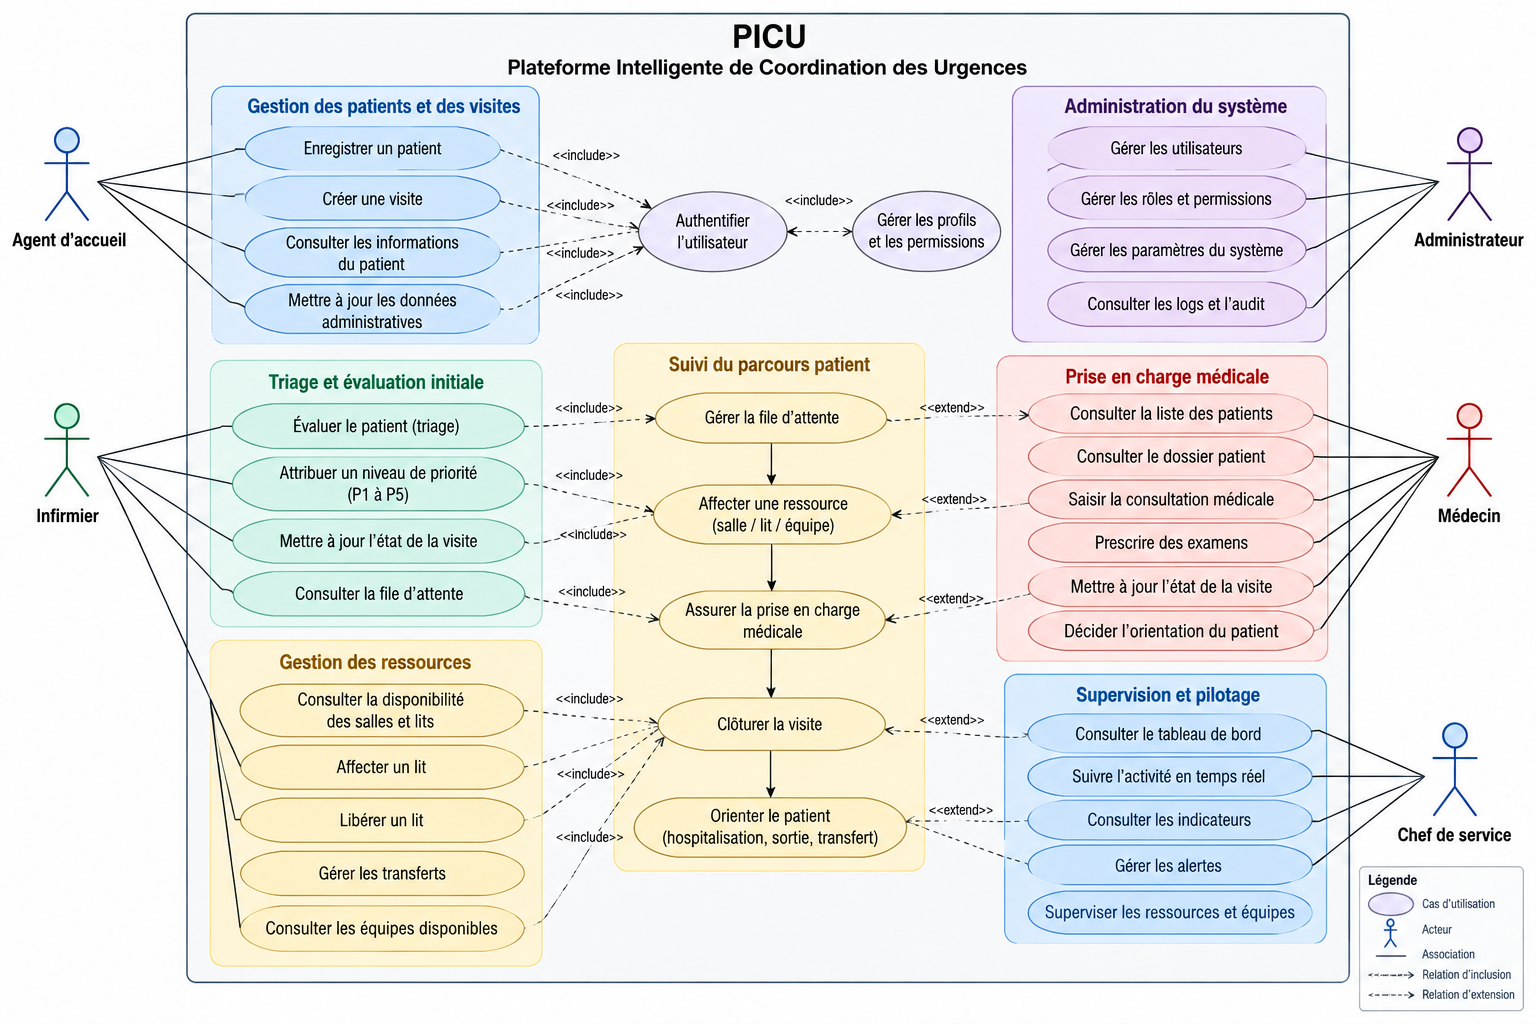
\includegraphics[width=0.9\textwidth]{images/use_case_diagram.png}}{\fbox{\parbox{0.9\textwidth}{\centering\vspace{1.5cm}À insérer : \texttt{images/use\_case\_diagram.png}\vspace{1.5cm}}}}
    \caption{Diagramme de cas d'utilisation de PICU}
    \label{fig:use_case_diagram}
\end{figure}

\section{Description des principaux cas d'utilisation}

\subsubsection{UC1 — Authentification et redirection par rôle}
\textbf{Acteur} : tous. Connexion par identifiants, émission d'un jeton JWT, redirection vers le tableau de bord du rôle.

\subsubsection{UC2 — Enregistrement d'un patient}
\textbf{Acteur} : Réceptionniste, Chef. Recherche par numéro national, création du patient et de la visite, priorité d'enregistrement et motif ; la visite entre en phase \texttt{triage\_pending}.

\subsubsection{UC3 — Triage clinique}
\textbf{Acteur} : Infirmier. Saisie d'une évaluation de triage (priorité, note, constantes, orientation), historique conservé.

\subsubsection{UC4 — Appel et placement}
\textbf{Acteur} : Réceptionniste, Infirmier. Appel du patient dans la file, puis affectation à une ressource compatible et libre.

\subsubsection{UC5 — Prise en charge médicale}
\textbf{Acteur} : Médecin, Infirmier. Démarrage de consultation, remplissage du dossier, clôture avec outcome.

\subsubsection{UC6 — Transfert et relève}
\textbf{Acteur} : Médecin, Infirmier, Chef. Demande de transfert de lit ou de relève, confirmée ou refusée selon les rôles autorisés.

\subsubsection{UC7 — Supervision}
\textbf{Acteur} : Chef. Consultation du pipeline, des indicateurs SLA et des alertes opérationnelles ; acquittement et résolution.

\subsubsection{UC8 — Assistance IA}
\textbf{Acteur} : Système IA, personnel habilité. Production de recommandations et, le cas échéant, proposition d'actions soumises à approbation.

\subsubsection{UC9 — Administration}
\textbf{Acteur} : Administrateur. Gestion des utilisateurs, des rôles et de la configuration (dont les paramètres IA).

\section{Matrice de traçabilité des exigences}

La rigueur d'ingénierie exige de relier chaque exigence à son implémentation et à sa validation. Le tableau suivant en donne un extrait (la matrice complète figure en annexe).

\begin{table}[H]
\centering
\caption{Extrait de la matrice Exigence $\rightarrow$ Implémentation $\rightarrow$ Test}
\label{tab:matrice}
\small
\begin{tabular}{|l|l|l|}
\hline
\textbf{Exigence} & \textbf{Implémentation} & \textbf{Validation} \\
\hline
Une seule visite active & \texttt{visitService.registerVisit} & Test d'intégrité / 409 \\
\hline
Un seul patient par lit & \texttt{assertBedAssignable}, verrou & Test concurrence / 409 \\
\hline
Transitions valides & \texttt{visitService}, \texttt{careStage} & Tests par rôle \\
\hline
Lit non affectable si « cleaning » & \texttt{resourceService} & \texttt{npm run test:v4} \\
\hline
Seuils SLA non approuvés inactifs & \texttt{supervisionRulesService} & \texttt{npm run test:supervision} \\
\hline
Indices d'enregistrement & \texttt{registrationHints} & \texttt{npm run test:registration} \\
\hline
Actions IA à risque approuvées & \texttt{action-policy} & Tests de politique IA \\
\hline
\end{tabular}
\end{table}

\section{Gestion des risques}

\begin{table}[H]
\centering
\caption{Risques identifiés et mesures de prévention}
\label{tab:risques}
\small
\begin{tabular}{|p{3.4cm}|p{5.6cm}|p{4.4cm}|}
\hline
\textbf{Risque} & \textbf{Mesure de prévention} & \textbf{Limite résiduelle} \\
\hline
Erreur de priorisation & Assistance IA supervisée + historique de triage & Précision IA perfectible \\
\hline
Conflit d'affectation d'un lit & Verrou \texttt{FOR UPDATE} + contrainte d'affectation unique & Dépend de la disponibilité réelle \\
\hline
Perte de connexion temps réel & Raisonnement par état serveur + rechargement & Latence possible des écrans \\
\hline
Confidentialité des données & RBAC, JWT, secrets hors dépôt & Pas d'audit externe réalisé \\
\hline
Décision automatisée abusive & Politique d'actions IA, approbation obligatoire, mode simulation restreint & Nécessite gouvernance continue \\
\hline
\end{tabular}
\end{table}

\section{Conclusion}

Les besoins sont formalisés en exigences fonctionnelles et non fonctionnelles, règles métier, cas d'utilisation, matrice de traçabilité et analyse de risques. Le chapitre suivant présente la méthodologie de développement et la conception du système.


% Chapitre 3 : Méthodologie et conception du système
\chapter{Méthodologie et conception du système}

\section{Introduction}

Ce chapitre présente d'abord la \textbf{méthodologie de développement} (organisation, itérations, gestion de versions), puis la \textbf{conception} : architecture logicielle, machine à états, modélisation UML, conception de la base de données et choix technologiques. Conformément à l'objectif du rapport, chaque choix technique est justifié.

\section{Méthodologie de développement}

\subsection{Démarche itérative et incrémentale}

Le projet a été conduit par itérations successives, chacune livrant un incrément testable :

\begin{enumerate}
    \item \textbf{Socle} : authentification, patients/visites, machine à états transactionnelle, boards ;
    \item \textbf{Enrichissement du parcours (V3)} : phases de soin, orientations, historique de triage, cycle des lits, examens et tâches ;
    \item \textbf{Supervision et ressources (V4)} : SLA, alertes, transferts, relèves, indicateurs de capacité ;
    \item \textbf{Assistance IA} : agents de triage, lits, capacité et documentation, sous supervision.
\end{enumerate}

\subsection{Organisation du travail et jalons}

Chaque incrément est matérialisé par une \textbf{migration SQL versionnée} (nommée \texttt{AAAAMMJJ\_description.sql}), ce qui rend l'évolution du schéma reproductible et auditables. Les jalons sont documentés dans le dépôt (plans, notes de passage de phase, rapports de test).

\subsection{Gestion des versions}

Le code est géré avec Git selon une convention de messages claire. Deux dispositifs garantissent l'hygiène du dépôt :

\begin{itemize}
    \item des \textbf{hooks pre-commit} (scripts locaux) qui bloquent les erreurs évidentes ;
    \item un \textbf{pipeline GitHub Actions} « secret guard » qui échoue si un fichier \texttt{.env} est versionné.
\end{itemize}

\section{Architecture logicielle}

\subsection{Architecture en trois couches}

PICU suit une architecture client-serveur en trois couches :

\begin{enumerate}
    \item \textbf{Présentation} : React~19 + Vite + TailwindCSS (tableaux de bord par rôle) ;
    \item \textbf{Application} : Node.js + Express (API REST + Socket.IO), services métier et middleware ;
    \item \textbf{Données} : PostgreSQL hébergé sur Neon.
\end{enumerate}

\subsection{Organisation des services backend}

Le backend est organisé en couches pour séparer les responsabilités :

\begin{itemize}
    \item \textbf{routes} (\texttt{*Routes.js}) : exposition HTTP, contrôle des capacités, validation d'entrée ;
    \item \textbf{services} (\texttt{*Service.js}) : logique métier transactionnelle (par exemple \texttt{visitService}, \texttt{resourceService}, \texttt{supervisionRulesService}, \texttt{transferRequestService}) ;
    \item \textbf{lib} : utilitaires transverses (par exemple \texttt{careStage}, journalisation d'actions) ;
    \item \textbf{middleware} : authentification (\texttt{authenticateJwt}), autorisation (\texttt{requireRole}, \texttt{requireCapability}) ;
    \item \textbf{ai} : agents, orchestrateur, fournisseur NIM, politiques d'action, observabilité.
\end{itemize}

\subsection{Communication REST et temps réel}

La communication combine des requêtes HTTP REST (JSON) et un canal temps réel \textbf{Socket.IO}. Le serveur diffuse des événements dérivés des transitions de visite (notamment \texttt{visit:status\_changed} et \texttt{queue:updated}) afin que tous les postes se synchronisent sans rechargement.

\begin{figure}[H]
    \centering
    % Image à déposer dans rapport-stage/images/ : architecture_picu.png
    \IfFileExists{images/architecture_picu.png}{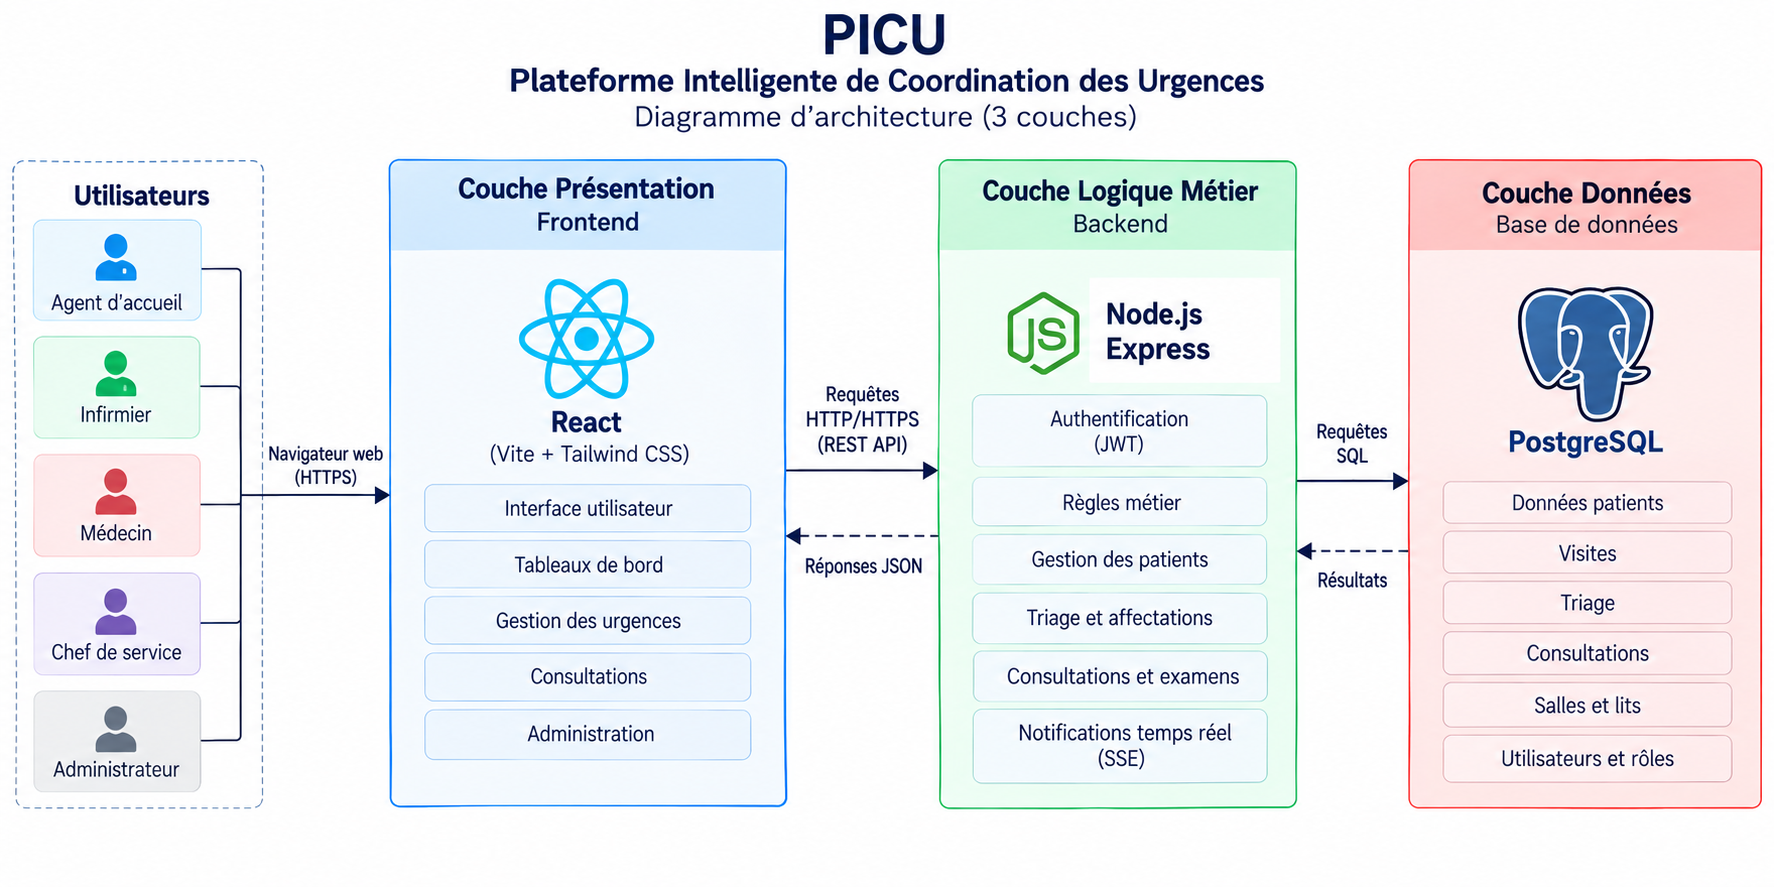
\includegraphics[width=0.92\textwidth]{images/architecture_picu.png}}{\fbox{\parbox{0.92\textwidth}{\centering\vspace{1.5cm}À insérer : \texttt{images/architecture\_picu.png}\vspace{1.5cm}}}}
    \caption{Architecture en trois couches et communications REST/Socket.IO}
    \label{fig:architecture_picu}
\end{figure}

\section{Conception du workflow : machine à états}

\subsection{États de la visite}

Le statut de la visite est la source de vérité du parcours. Il se décompose en trois états principaux et trois états terminaux.

\begin{table}[H]
\centering
\caption{Machine à états du statut de visite}
\label{tab:etats}
\small
\begin{tabular}{|l|l|l|}
\hline
\textbf{Statut} & \textbf{Signification} & \textbf{Transitions sortantes} \\
\hline
\texttt{waiting} & Enregistré, en attente de prise en charge & \texttt{place}, \texttt{close} (parti avant) \\
\hline
\texttt{placed} & Affecté à une ressource & \texttt{start}, \texttt{return}, \texttt{close} \\
\hline
\texttt{in\_treatment} & Prise en charge en cours & \texttt{close} \\
\hline
\texttt{discharged} & Sortie autorisée (terminal) & --- \\
\hline
\texttt{transferred} & Transféré (terminal) & --- \\
\hline
\texttt{left\_without\_seen} & Parti avant prise en charge (terminal) & --- \\
\hline
\end{tabular}
\end{table}

\subsection{Actions et transitions}

Chaque action est une transition atomique exécutée dans une transaction. Le tableau suivant résume les actions autorisées et leurs effets.

\begin{table}[H]
\centering
\caption{Actions de workflow et règles}
\label{tab:actions}
\small
\begin{tabular}{|l|l|l|p{5.4cm}|}
\hline
\textbf{Action} & \textbf{De} & \textbf{Vers} & \textbf{Effet principal} \\
\hline
\texttt{register} & --- & \texttt{waiting} & Crée patient + visite, une seule visite active \\
\hline
\texttt{call} & \texttt{waiting} & \texttt{waiting} & Horodate l'appel, incrémente le compteur \\
\hline
\texttt{place} & \texttt{waiting} & \texttt{placed} & Occupe une ressource libre et compatible \\
\hline
\texttt{return} & \texttt{placed} & \texttt{waiting} & Libère la ressource, remet en file \\
\hline
\texttt{start} & \texttt{placed} & \texttt{in\_treatment} & Ouvre la consultation \\
\hline
\texttt{close} & \texttt{placed}/\texttt{in\_treatment} & terminal & Libère la ressource, fixe l'outcome \\
\hline
\texttt{triage} & \texttt{waiting} & \texttt{waiting} & Enregistre une évaluation de triage \\
\hline
\end{tabular}
\end{table}

\subsection{Dimension multi-états}

Au-delà du statut, la visite porte des dimensions orthogonales qui permettent un suivi fin : la \textbf{phase de soin} (\texttt{care\_stage} : \texttt{registered}, \texttt{triage\_pending}, \texttt{waiting\_care}, \texttt{in\_care}, \texttt{in\_observation}, \texttt{disposition\_pending}, \texttt{completed}), l'\textbf{orientation} (\texttt{critical}, \texttt{acute}, \texttt{standard}, \texttt{ambulatory}, \texttt{observation}, \texttt{isolation}), la \textbf{localisation} du patient et le \textbf{code public}.

\subsection{Conception de la concurrence}

Le point critique est l'affectation des ressources. La solution retenue combine :

\begin{enumerate}
    \item un verrou de ligne sur la visite (\texttt{SELECT ... FOR UPDATE}) ;
    \item une vérification qu'aucune affectation active n'existe pour la ressource ni pour la visite ;
    \item une insertion d'affectation et une mise à jour de statut dans la \textbf{même transaction}.
\end{enumerate}

Ainsi, deux infirmiers qui tentent d'affecter le même lit simultanément voient l'un réussir et l'autre échouer avec un conflit (HTTP~409), sans jamais produire d'état incohérent.

\section{Diagrammes UML}

\subsection{Diagramme de séquence — enregistrement}

\begin{figure}[H]
    \centering
    % Image à déposer dans rapport-stage/images/ : sequence_diagram.png
    \IfFileExists{images/sequence_diagram.png}{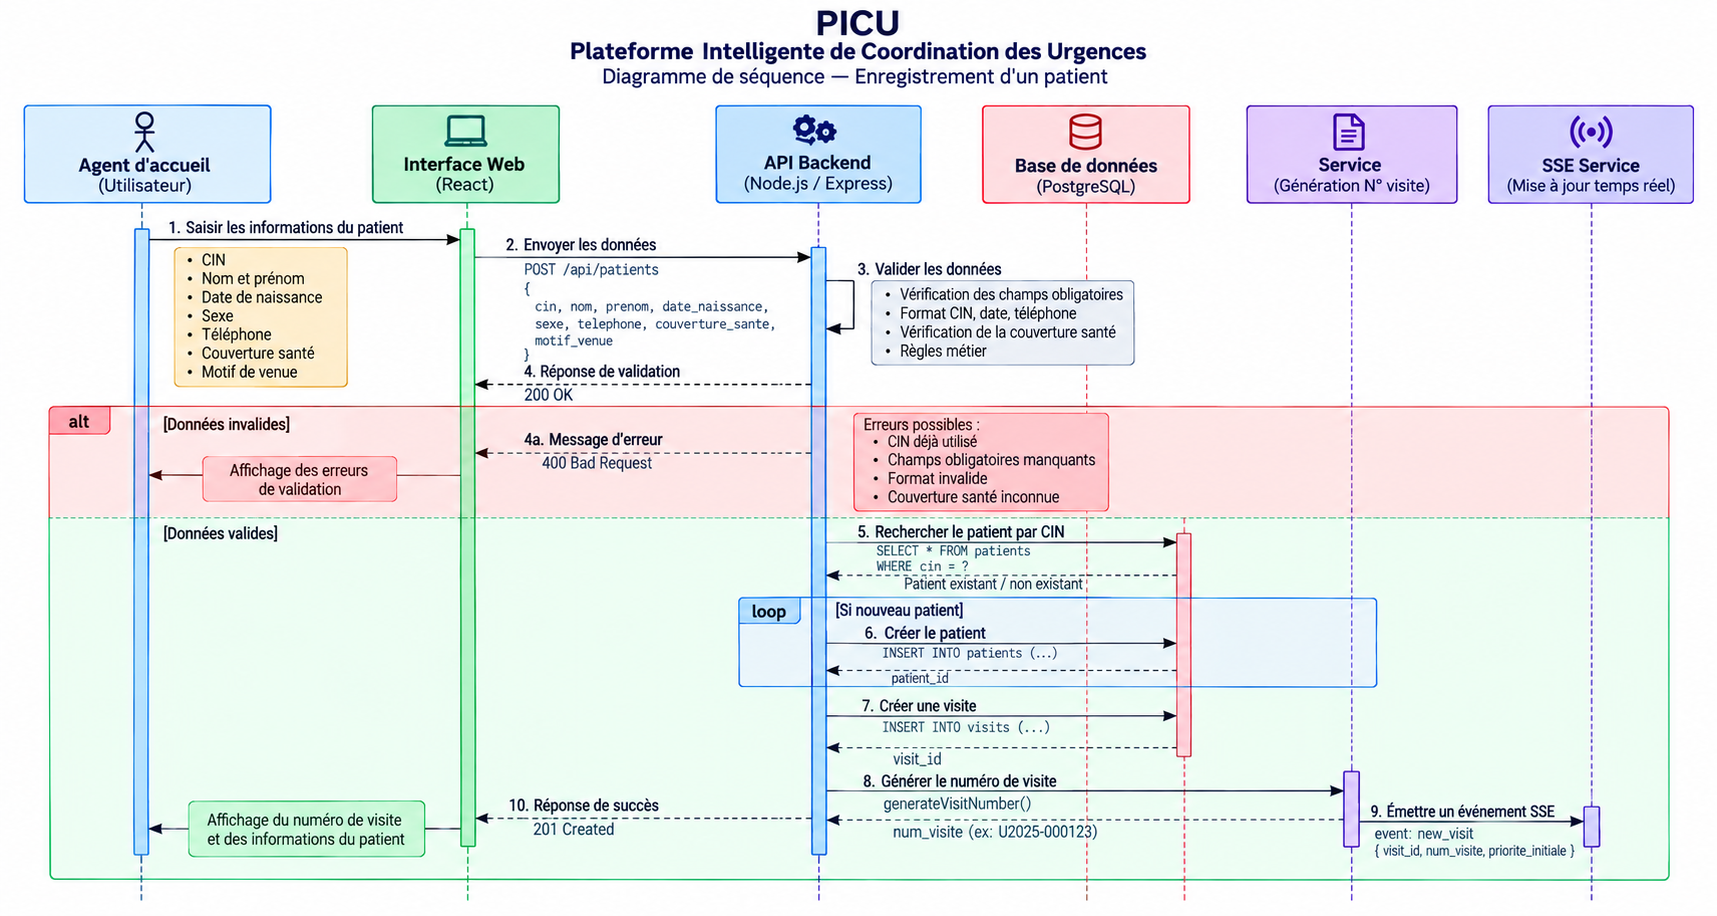
\includegraphics[width=0.9\textwidth]{images/sequence_diagram.png}}{\fbox{\parbox{0.9\textwidth}{\centering\vspace{1.5cm}À insérer : \texttt{images/sequence\_diagram.png}\vspace{1.5cm}}}}
    \caption{Diagramme de séquence — Enregistrement d'un patient}
    \label{fig:sequence_diagram}
\end{figure}

\subsection{Diagramme d'activité — circuit de triage}

\begin{figure}[H]
    \centering
    % Image à déposer dans rapport-stage/images/ : activity_diagram.png
    \IfFileExists{images/activity_diagram.png}{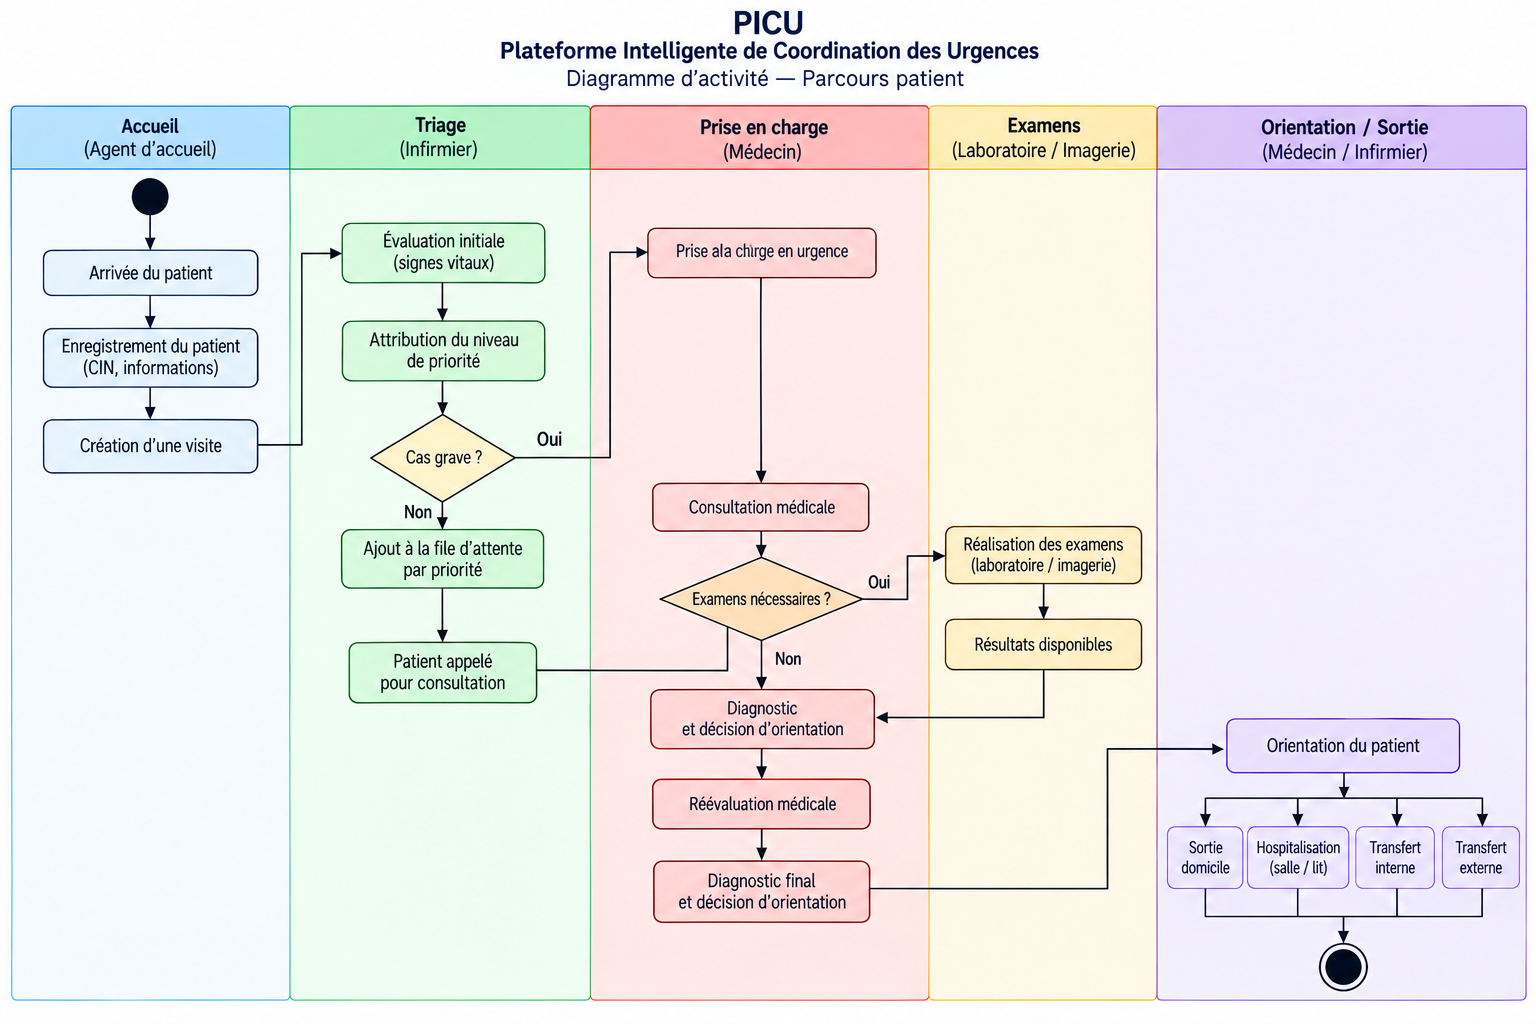
\includegraphics[width=0.9\textwidth]{images/activity_diagram.png}}{\fbox{\parbox{0.9\textwidth}{\centering\vspace{1.5cm}À insérer : \texttt{images/activity\_diagram.png}\vspace{1.5cm}}}}
    \caption{Diagramme d'activité — Circuit de triage et de prise en charge}
    \label{fig:activity_diagram}
\end{figure}

\subsection{Diagramme de classes}

\begin{figure}[H]
    \centering
    % Image à déposer dans rapport-stage/images/ : class_diagram.png
    \IfFileExists{images/class_diagram.png}{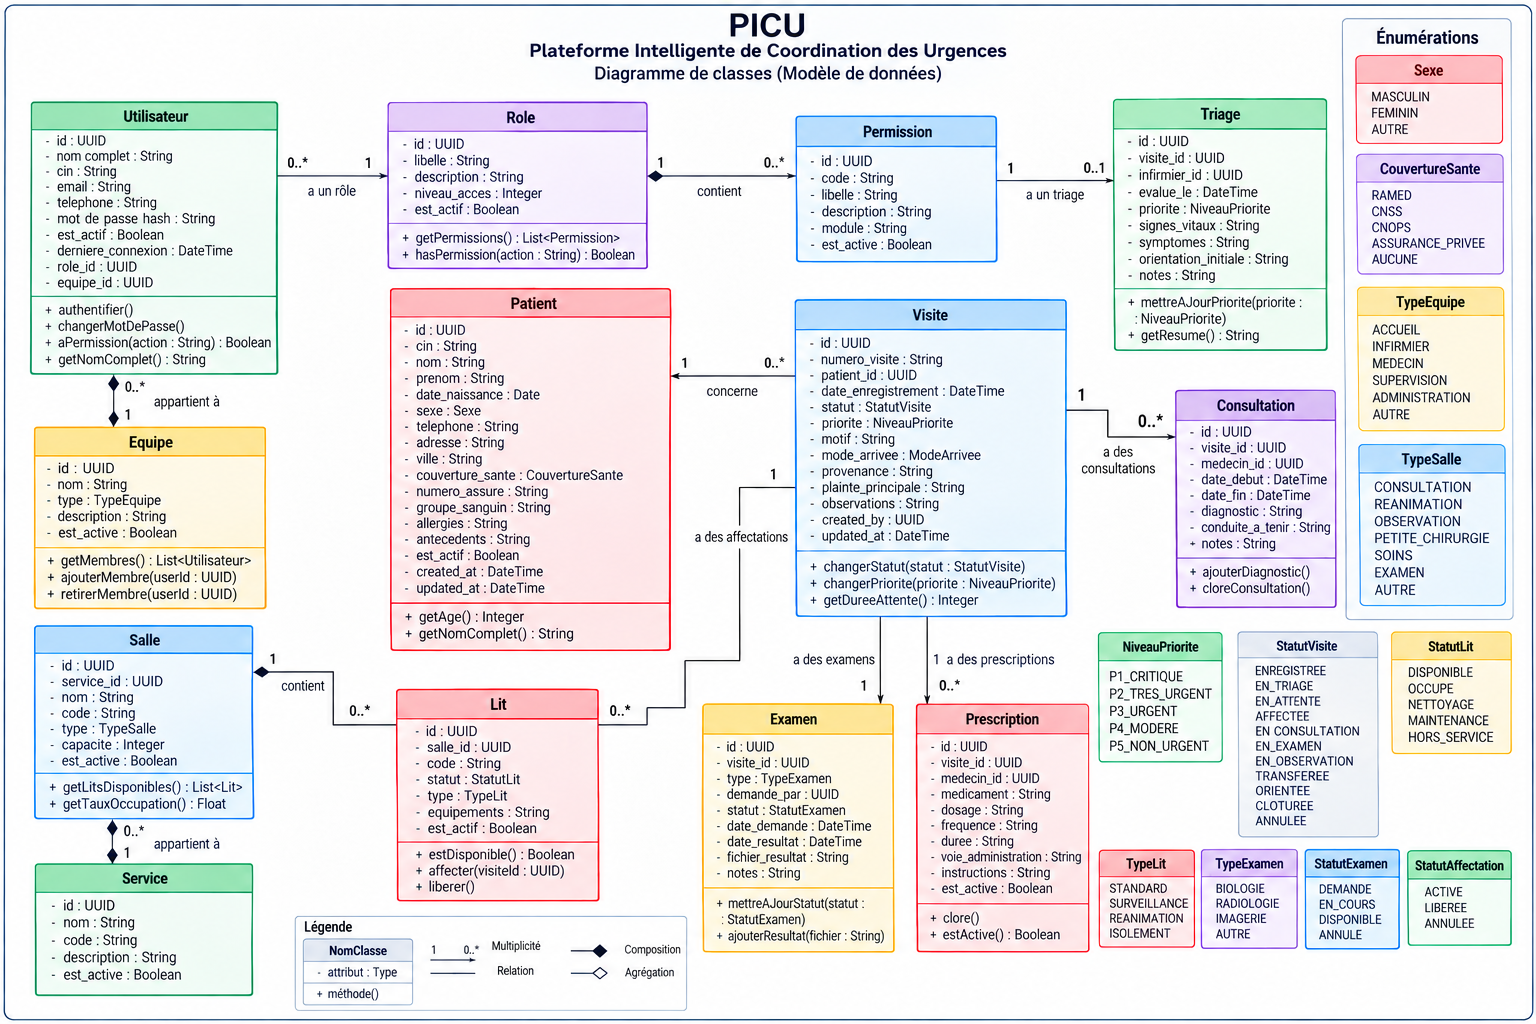
\includegraphics[width=0.9\textwidth]{images/class_diagram.png}}{\fbox{\parbox{0.9\textwidth}{\centering\vspace{1.5cm}À insérer : \texttt{images/class\_diagram.png}\vspace{1.5cm}}}}
    \caption{Diagramme de classes de PICU}
    \label{fig:class_diagram}
\end{figure}

\section{Conception de la base de données}

\subsection{Modèle relationnel}

La base repose sur un schéma relationnel normalisé (3FN). Les entités principales sont : \texttt{users}, \texttt{patients}, \texttt{visits}, \texttt{zones}, \texttt{rooms}, \texttt{beds}, \texttt{bed\_assignments}, \texttt{consultations}, \texttt{triage\_assessments}, \texttt{exams}, \texttt{care\_tasks}, \texttt{visit\_events}, \texttt{room\_teams}, \texttt{resource\_status\_events}, ainsi que les tables V4 (\texttt{transfer\_requests}, \texttt{handoff\_requests}, \texttt{operational\_alerts}, \texttt{workflow\_settings}) et IA (\texttt{agent\_runs}, \texttt{agent\_recommendations}, \texttt{agent\_actions}, \texttt{agent\_approvals}).

\subsection{Contraintes d'intégrité}

L'intégrité est assurée au niveau du schéma par :

\begin{itemize}
    \item des \textbf{clés étrangères} avec politiques de suppression restrictives pour les entités critiques ;
    \item des \textbf{contraintes de domaine} (\texttt{CHECK}) sur les statuts, phases, orientations, outcomes et statuts opérationnels ;
    \item des \textbf{index uniques} empêchant un doublon de code public ou d'affectation active ;
    \item des \textbf{vues} (\texttt{waiting\_board}, \texttt{bed\_board}) exposant l'état consolidé.
\end{itemize}

\subsection{Dictionnaire de données (extrait)}

\begin{table}[H]
\centering
\caption{Dictionnaire de données — extrait}
\label{tab:data_dictionary}
\small
\begin{tabular}{|l|l|p{6cm}|}
\hline
\textbf{Table} & \textbf{Colonne} & \textbf{Description} \\
\hline
visit\_events & event\_type & Type d'événement (enregistré, appelé, placé, triage, clôturé...) \\
\hline
 & actor\_type & \texttt{user}, \texttt{agent} ou \texttt{system} \\
\hline
 & idempotency\_key & Clé unique garantissant la non-duplication d'une action \\
\hline
visits & status & Statut de la machine à états \\
\hline
 & care\_stage & Phase de soin \\
\hline
 & current\_orientation & Orientation clinique courante \\
\hline
beds & resource\_type \texttt{/} operational\_status & Type (lit, fauteuil, box...) et état opérationnel \\
\hline
triage\_assessments & assessment\_type & \texttt{initial}, \texttt{reassessment} ou \texttt{escalation} \\
\hline
transfer\_requests & status & \texttt{pending}, \texttt{confirmed}, \texttt{cancelled}, \texttt{expired} \\
\hline
agent\_actions & requires\_approval & Indique si l'action IA doit être approuvée \\
\hline
\end{tabular}
\end{table}

\subsection{Stratégie de migration}

Chaque évolution est apportée par une migration additive et idempotente (\texttt{ADD COLUMN IF NOT EXISTS}, \texttt{CREATE TABLE IF NOT EXISTS}) appliquée par un script dédié (\texttt{npm run migrate:v3}, \texttt{migrate:v4}, \texttt{migrate:ai}). Cette stratégie permet de faire évoluer un schéma en production sans rupture.

\section{Choix technologiques et justification}

\begin{table}[H]
\centering
\caption{Choix technologiques et justification}
\label{tab:choix}
\small
\begin{tabular}{|l|l|p{6.4cm}|}
\hline
\textbf{Brique} & \textbf{Technologie} & \textbf{Justification} \\
\hline
Frontend & React 19 + Vite & Écosystème mature, composants réutilisables, build rapide. \\
\hline
Style & TailwindCSS & Cohérence visuelle et rapidité de prototypage. \\
\hline
Backend & Node.js + Express & Même langage que le frontend, middleware simple. \\
\hline
Base & PostgreSQL (Neon) & Intégrité relationnelle, transactions, JSONB, gestion managée. \\
\hline
Temps réel & Socket.IO & Diffusion d'événements, repli polling. \\
\hline
Auth & JWT + bcrypt & Standard, sans session serveur. \\
\hline
IA & NVIDIA NIM & Modèles spécialisés, sorties structurées (JSON schema). \\
\hline
\end{tabular}
\end{table}

\section{Conclusion}

La méthode itérative, une architecture en couches, une machine à états explicite et une base fortement contrainte constituent le socle de PICU. Le chapitre suivant détaille la réalisation concrète de ces choix.


% Chapitre 4 : Réalisation de la plateforme PICU
\chapter{Réalisation de la plateforme PICU}

\section{Introduction}

Ce chapitre décrit la réalisation concrète des choix de conception. Il présente l'environnement de développement, puis chaque module du parcours patient, les interfaces, la communication temps réel et la couche d'assistance IA. Pour chaque module, la logique métier et sa traduction technique sont explicitées.

\section{Environnement de développement}

\subsection{Technologies}

React~19, Vite, TailwindCSS, React Router, Node.js, Express, PostgreSQL (Neon), Socket.IO, JWT, bcrypt, NVIDIA NIM (SDK compatible OpenAI), \texttt{node:test}.

\subsection{Outils}

Visual Studio Code, Git, GitHub Actions, Chrome/Firefox (DevTools), Draw.io / Mermaid, pgAdmin/psql.

\section{Module d'authentification et de gestion des accès}

L'authentification est implémentée dans les routes d'authentification et le middleware \texttt{authenticateJwt}. Le mot de passe est haché avec bcrypt ; la connexion émet un jeton JWT stocké côté client. À chaque requête, le middleware recharge l'utilisateur en base et rejette tout compte inactif. L'autorisation combine deux niveaux : un contrôle par \textbf{rôle} (\texttt{requireRole}) et un contrôle plus fin par \textbf{capacité} (\texttt{requireCapability}).

\begin{table}[H]
\centering
\caption{Capacités par rôle (extrait)}
\label{tab:roles}
\small
\begin{tabular}{|l|p{9.4cm}|}
\hline
\textbf{Rôle} & \textbf{Capacités} \\
\hline
Réceptionniste & register, call, critical \\
\hline
Infirmier & place, return, start, fill, close, triage, critical, ai\_documentation, ai\_triage\_recommend, ai\_bed\_flow \\
\hline
Médecin & start, close, fill, ai\_documentation, ai\_triage\_recommend \\
\hline
Chef & register, call, place, start, return, close, fill, critical, ai\_health, ai\_settings, + IA \\
\hline
Administrateur & manage\_users, ai\_health, ai\_settings \\
\hline
\end{tabular}
\end{table}

\begin{figure}[H]
    \centering
    % Image à déposer dans rapport-stage/images/ : login_screen.png
    \IfFileExists{images/login_screen.png}{\includegraphics[width=0.8\textwidth]{images/login_screen.png}}{\fbox{\parbox{0.8\textwidth}{\centering\vspace{1.5cm}À insérer : \texttt{images/login\_screen.png}\vspace{1.5cm}}}}
    \caption{Page de connexion de PICU}
    \label{fig:login_screen}
\end{figure}

\section{Module patients et visites}

Les routes de visite exposent les actions du workflow. L'enregistrement crée le patient s'il est inconnu (recherche par numéro national), vérifie qu'aucune visite active n'existe, puis crée la visite avec un \textbf{code public unique} et la place en phase de triage. Un mécanisme d'\textbf{idempotence} (clé fournie par le client) garantit qu'un double envoi ne crée pas deux visites.

Chaque action suit le même patron : ouverture d'une transaction, verrouillage de la visite, contrôle de l'état courant, écriture métier, journalisation d'un événement \texttt{visit\_events}, puis validation de la transaction.

\section{Module file d'attente et appel}

La file d'attente n'est pas stockée comme une table mutable : elle est \textbf{calculée} à la lecture par une vue (\texttt{waiting\_board}) qui ordonne les patients par priorité croissante, indicateur critique puis date d'arrivée. La position est donc cohérente sans risque de doublons.

L'action \texttt{call} reste dans l'état \texttt{waiting} : elle enregistre l'heure du dernier appel et incrémente un compteur, matérialisant visuellement qu'un patient « a été appelé » sans le retirer de la file. Le staff de chaque rôle dispose de vues de travail (\texttt{/queue/worklists}) filtrées selon son périmètre.

\section{Module de triage}

Le triage est structuré et historisé. Chaque évaluation est enregistrée dans \texttt{triage\_assessments} avec sa priorité (1--5), son type (\texttt{initial}, \texttt{reassessment}, \texttt{escalation}), une note clinique, des constantes éventuelles (JSONB), une orientation et, en cas de changement, un motif. Un indicateur \texttt{critical\_flag} peut être posé pour le fast-track des patients critiques.

Le système distingue explicitement la \textbf{priorité d'enregistrement} (fixée à l'accueil) et la \textbf{priorité clinique} (validée au triage), ce qui permet de mesurer l'apport du triage et d'éviter de confondre les deux notions.

\section{Module de gestion des ressources}

\subsection{Typologie et cycle de vie}

Une ressource est un lit typé (\texttt{resource\_type} : lit, fauteuil, box, poste de triage, poste de consultation) associé à une salle et à une zone. Elle possède un \textbf{état opérationnel} (\texttt{ready}, \texttt{cleaning}, \texttt{maintenance}, \texttt{blocked}, \texttt{out\_of\_service}). Les transitions d'état sont tracées dans \texttt{resource\_status\_events}, et le passage direct de « nettoyage » à « prêt » est refusé pour imposer un contrôle humain de remise en service.

\subsection{Affectation et libération}

L'affectation vérifie que la ressource est affectable (\texttt{assertBedAssignable}), qu'aucune affectation active n'existe, puis crée l'affectation et passe la visite en \texttt{placed}. À la clôture ou au retour, la ressource est libérée et bascule en \textbf{turnover} (nettoyage) avant remise à disposition.

\subsection{Le plan des lits}

L'interface \texttt{BedPlanPanel} présente les zones, salles et lits avec leur occupation, et permet l'affectation d'un lit libre. Elle est partagée par l'infirmier, le médecin et le chef, avec des droits différents.

\begin{figure}[H]
    \centering
    % Image à déposer dans rapport-stage/images/ : dashboard_infirmier.png
    \IfFileExists{images/dashboard_infirmier.png}{\includegraphics[width=0.9\textwidth]{images/dashboard_infirmier.png}}{\fbox{\parbox{0.9\textwidth}{\centering\vspace{1.5cm}À insérer : \texttt{images/dashboard\_infirmier.png}\vspace{1.5cm}}}}
    \caption{Dashboard Infirmier — triage, plan des lits et file}
    \label{fig:dashboard_infirmier}
\end{figure}

\section{Module de prise en charge et consultations}

Le démarrage d'une consultation crée une ligne \texttt{consultations} (médecin attribué, auteur de la saisie), passe la visite en \texttt{in\_treatment} et en phase \texttt{in\_care}. Le remplissage met à jour diagnostic et notes ; la clôture libère la ressource, clôture la consultation et fixe l'\textbf{outcome} (sortie, hospitalisation, transfert, parti avant ou pendant la prise en charge). Les règles d'accès garantissent qu'un médecin ne gère que les patients de sa salle et qu'un infirmier ne rédige que pour le médecin référent de la salle.

\begin{figure}[H]
    \centering
    % Image à déposer dans rapport-stage/images/ : dashboard_medecin.png
    \IfFileExists{images/dashboard_medecin.png}{\includegraphics[width=0.9\textwidth]{images/dashboard_medecin.png}}{\fbox{\parbox{0.9\textwidth}{\centering\vspace{1.5cm}À insérer : \texttt{images/dashboard\_medecin.png}\vspace{1.5cm}}}}
    \caption{Dashboard Médecin — patients actifs et consultations}
    \label{fig:dashboard_medecin}
\end{figure}

\section{Module transferts, relèves, examens et tâches}

\subsection{Transferts de lit}

Une demande de transfert (\texttt{transfer\_requests}) décrit le lit source, le lit cible et un statut (\texttt{pending}, \texttt{confirmed}, \texttt{cancelled}, \texttt{expired}). La confirmation n'est autorisée qu'à certains rôles et déclenche le déplacement effectif, tracé par un événement.

\subsection{Relèves}

Une demande de relève (\texttt{handoff\_requests}) formalise le passage de responsabilité d'un soignant à un autre, avec motif et statut (\texttt{pending}, \texttt{accepted}, \texttt{declined}, \texttt{cancelled}).

\subsection{Examens et tâches de soin}

Les tables \texttt{exams} et \texttt{care\_tasks} permettent de demander des examens (biologie, imagerie) et de créer des tâches de soin, avec statuts et horodatages, l'ensemble étant journalisé et visible dans le dossier de la visite.

\section{Module supervision et alertes}

Le chef de service dispose d'un centre de commande (\textit{command center}) qui agrège :

\begin{itemize}
    \item le \textbf{pipeline} des patients par étape ;
    \item les \textbf{indicateurs SLA} et la détection de patients bloqués ;
    \item les \textbf{alertes opérationnelles} hiérarchisées ;
    \item les indicateurs de \textbf{capacité} et de charge ;
    \item les \textbf{équipes de salle} et le plan des lits.
\end{itemize}

\subsection{Seuils SLA}

Les seuils de blocage sont configurables ; les valeurs par défaut sont présentées ci-dessous. Chaque dépassement est qualifié de \textit{warning} ou de \textit{critical} selon un facteur deux.

\begin{table}[H]
\centering
\caption{Seuils SLA par défaut (chef de service)}
\label{tab:sla}
\small
\begin{tabular}{|l|c|}
\hline
\textbf{Situation} & \textbf{Seuil (minutes)} \\
\hline
Attente non appelé & 20 \\
\hline
Appelé sans mise au lit & 15 \\
\hline
Au lit sans consultation & 30 \\
\hline
Prise en charge prolongée & 60 \\
\hline
\end{tabular}
\end{table}

\subsection{Règles de supervision}

Les règles de supervision sont pilotées par des paramètres (\texttt{workflow\_settings}). Par prudence, une règle de délai n'est active que si elle est explicitement \textbf{approuvée} (le test \texttt{ruleConfigured} le vérifie). Les règles de réévaluation périodique et de pression de capacité sont activées ; les seuils de délai non validés restent désactivés en attente de validation par l'établissement.

\subsection{Alertes opérationnelles}

Les alertes (\texttt{operational\_alerts}) possèdent un cycle de vie (\texttt{open}, \texttt{acknowledged}, \texttt{resolved}, \texttt{obsolete}), une sévérité, une déduplication par clé et un historique d'événements. Leur évaluation est déclenchée périodiquement par le serveur.

\begin{figure}[H]
    \centering
    % Image à déposer dans rapport-stage/images/ : dashboard_chef.png
    \IfFileExists{images/dashboard_chef.png}{\includegraphics[width=0.9\textwidth]{images/dashboard_chef.png}}{\fbox{\parbox{0.9\textwidth}{\centering\vspace{1.5cm}À insérer : \texttt{images/dashboard\_chef.png}\vspace{1.5cm}}}}
    \caption{Dashboard Chef de service — centre de commande}
    \label{fig:dashboard_chef}
\end{figure}

\section{Tableaux de bord par rôle}

Chaque rôle dispose d'un tableau de bord dédié :

\begin{itemize}
    \item \textbf{Accueil} : enregistrement, file, KPI, appel ;
    \item \textbf{Infirmier} : triage, plan des lits, file, tâches ;
    \item \textbf{Médecin} : charge de travail, salle, consultations ;
    \item \textbf{Chef} : pipeline, SLA, alertes, capacité, équipes ;
    \item \textbf{Administrateur} : utilisateurs, rôles, configuration.
\end{itemize}

\begin{figure}[H]
    \centering
    % Image à déposer dans rapport-stage/images/ : dashboard_receptionniste.png
    \IfFileExists{images/dashboard_receptionniste.png}{\includegraphics[width=0.9\textwidth]{images/dashboard_receptionniste.png}}{\fbox{\parbox{0.9\textwidth}{\centering\vspace{1.5cm}À insérer : \texttt{images/dashboard\_receptionniste.png}\vspace{1.5cm}}}}
    \caption{Dashboard Accueil — file d'attente et enregistrement}
    \label{fig:dashboard_receptionniste}
\end{figure}

\begin{figure}[H]
    \centering
    % Image à déposer dans rapport-stage/images/ : dashboard_admin.png
    \IfFileExists{images/dashboard_admin.png}{\includegraphics[width=0.9\textwidth]{images/dashboard_admin.png}}{\fbox{\parbox{0.9\textwidth}{\centering\vspace{1.5cm}À insérer : \texttt{images/dashboard\_admin.png}\vspace{1.5cm}}}}
    \caption{Dashboard Administrateur — configuration du système}
    \label{fig:dashboard_admin}
\end{figure}

\section{Synchronisation temps réel}

À chaque transition importante, le backend publie un événement Socket.IO. Les interfaces écoutent ces événements et se rafraîchissent sans rechargement de page, un \textbf{repli par interrogation périodique} assurant la résilience en cas de coupure du canal.

\begin{table}[H]
\centering
\caption{Principaux événements temps réel}
\label{tab:evenements}
\small
\begin{tabular}{|l|p{8.6cm}|}
\hline
\textbf{Événement} & \textbf{Déclencheur} \\
\hline
\texttt{visit:status\_changed} & Enregistrement, placement, prise en charge, clôture \\
\hline
\texttt{queue:updated} & Appel, placement, retour en file, nouvelle arrivée \\
\hline
\texttt{visit:timeline\_updated} & Nouvel événement de visite (audit) \\
\hline
\texttt{resource:status\_changed} & Changement d'état d'une ressource (nettoyage, prêt) \\
\hline
\end{tabular}
\end{table}

\section{Couche d'assistance IA}

\subsection{Objectifs et principes}

La couche IA vise à assister les équipes sans jamais décider à leur place. Quatre intentions sont supportées : \textbf{triage}, \textbf{flux de lits}, \textbf{capacité} et \textbf{documentation}. Chaque appel produit une exécution tracée (\texttt{agent\_runs}) et une recommandation (\texttt{agent\_recommendations}).

\subsection{Fournisseur et routage des modèles}

L'accès aux modèles passe par NVIDIA NIM. Un routeur de modèles associe à chaque tâche un profil : \textit{reasoning} pour le triage et la documentation, \textit{fast} pour les lits et la capacité, \textit{embedding} pour la recherche documentaire. Les sorties sont contraintes par des schémas JSON.

\subsection{Mode d'exécution et supervision}

Le mode IA est globalement configurable : \texttt{disabled}, \texttt{collaborative}, \texttt{supervised\_autonomy}, \texttt{full\_control\_simulation}. Des indicateurs par agent (documentation, triage, triage « shadow », lits, capacité) permettent d'activer sélectivement chaque fonction.

\subsection{Politique d'action et approbations}

Toute action IA est soumise à une \textbf{politique de risque} : les actions cliniques (triage, clôture) sont à risque maximal et exigent une approbation humaine ; seules quelques actions à faible risque (créer une tâche de réévaluation, rafraîchir une liste, lever une alerte) sont automatiques en mode supervisé. Un garde-fou interdit le mode « simulation » sur des visites réelles.

\begin{table}[H]
\centering
\caption{Politique d'actions IA (extrait)}
\label{tab:ai-actions}
\small
\begin{tabular}{|l|c|c|}
\hline
\textbf{Outil} & \textbf{Risque} & \textbf{Approbation requise} \\
\hline
triage & critique & oui \\
\hline
close & critique & oui \\
\hline
place / transfer & haut & oui \\
\hline
call / return & moyen & oui \\
\hline
createReassessmentTask & faible & non (mode supervisé) \\
\hline
raiseOperationalAlert & faible & non (mode supervisé) \\
\hline
\end{tabular}
\end{table}

\subsection{Mode « shadow » du triage}

Pour évaluer le triage IA sans risque, un mode « shadow » permet d'exécuter une recommandation en arrière-plan lors de l'enregistrement, sans l'afficher comme décision officielle. Cela permet de comparer, hors production, la proposition IA à la décision humaine.

\section{Conclusion}

L'ensemble du parcours patient est implémenté, de l'accueil à la clôture, avec des modules avancés de supervision, de ressources et d'assistance IA. Le chapitre suivant traite de l'assurance qualité, de la sécurité et de l'industrialisation.


% Chapitre 5 : Assurance qualité, sécurité et CI/CD
\chapter{Assurance qualité, sécurité et CI/CD}

\section{Introduction}

Ce chapitre traite d'un axe souvent négligé dans les rapports de stage : la \textbf{vérification de la qualité}, la \textbf{sécurité} et l'\textbf{industrialisation}. Nous présentons la stratégie de test et les résultats réellement obtenus, les mécanismes de sécurité et d'intégrité, puis la chaîne d'intégration et de livraison continue.

\section{Stratégie de test}

\subsection{Niveaux de test}

La stratégie combine plusieurs niveaux complémentaires :

\begin{itemize}
    \item \textbf{tests unitaires} : fonctions pures de règles (supervision, indices d'enregistrement) ;
    \item \textbf{tests d'intégrité} : invariants de ressources et transitions, exécutés contre une base isolée ;
    \item \textbf{tests fonctionnels} : parcours par rôle (accueil, infirmier, médecin, chef) ;
    \item \textbf{tests de concurrence} : affectation simultanée d'une même ressource ;
    \item \textbf{tests de bout en bout} : scénario complet du parcours patient.
\end{itemize}

\subsection{Outillage}

Les tests automatisés s'appuient sur le lanceur natif de Node.js (\texttt{node:test}) et \texttt{node:assert}, sans dépendance à un framework externe. Ils sont exécutés via des scripts npm (\texttt{test:v4}, \texttt{test:supervision}, \texttt{test:registration}). Un \textit{benchmark} de triage (\texttt{benchmarks/run-triage-benchmark.js}) mesure la latence du modèle NIM et enregistre ses résultats.

\section{Tests automatisés et résultats}

\subsection{Invariants de ressources — \texttt{npm run test:v4}}

Ce test vérifie trois invariants du cycle de vie des lits :

\begin{enumerate}
    \item une ressource en \textbf{nettoyage} ne peut être affectée (rejet HTTP~409) ;
    \item la libération d'une ressource la bascule en \textbf{nettoyage} (et non directement en « prêt ») ;
    \item la transition directe vers « prêt » est refusée (HTTP~422), imposant le contrôle de remise en service.
\end{enumerate}

\subsection{Règles de supervision — \texttt{npm run test:supervision}}

Ce test vérifie que \texttt{ruleConfigured} n'active \textbf{jamais} un seuil de délai qui n'est pas approuvé : une règle activée sans approbation est considérée inactive, garantissant qu'aucune alerte SLA non validée ne soit émise.

\subsection{Intelligence d'enregistrement — \texttt{npm run test:registration}}

Ce test vérifie que les \textbf{indices d'enregistrement} signalent un motif à risque, une arrivée en ambulance ou une priorité d'enregistrement élevée, sans jamais modifier la priorité clinique.

\subsection{Analytique patient}

Le module analytique dispose de son propre test vérifiant la cohérence des agrégats.

\begin{table}[H]
\centering
\caption{Matrice de tests — extrait}
\label{tab:tests}
\small
\begin{tabular}{|l|l|l|l|}
\hline
\textbf{ID} & \textbf{Scénario} & \textbf{Résultat attendu} & \textbf{Statut} \\
\hline
T1 & Affecter un lit en nettoyage & Rejet (409) & OK \\
\hline
T2 & Libérer un lit & Passe en nettoyage & OK \\
\hline
T3 & Forcer « prêt » sans contrôle & Rejet (422) & OK \\
\hline
T4 & Seuil SLA non approuvé & Inactif & OK \\
\hline
T5 & Indice motif critique & Suggestion sans mutation & OK \\
\hline
T6 & Double affectation du même lit & Un succès, un conflit (409) & OK \\
\hline
T7 & Double enregistrement (idempotence) & Une seule visite & OK \\
\hline
T8 & Parcours E2E complet & Transitions cohérentes & OK \\
\hline
\end{tabular}
\end{table}

\section{Cas d'étude : concurrence sur l'affectation d'un lit}

\subsection{Le problème}

Deux infirmiers consultent un même lit libre et cliquent « Affecter » au même instant. Sans précaution, deux patients pourraient se retrouver sur le même lit.

\subsection{La solution retenue et sa vérification}

L'affectation s'exécute dans une transaction : la visite est verrouillée (\texttt{SELECT ... FOR UPDATE}), l'absence d'affectation active est vérifiée, puis l'affectation est insérée et le statut mis à jour. Deux transactions concurrentes sont sérialisées par le verrou : la seconde détecte l'occupation et échoue proprement avec un conflit. Ce comportement est décrit par le test~T6.

\section{Tests fonctionnels et bout en bout}

Les parcours par rôle ont été validés manuellement et par scénario : enregistrement à l'accueil, triage infirmier, appel et placement, prise en charge et clôture. Le scénario de référence (documenté dans le dépôt) vérifie que chaque transition produit l'événement attendu dans \texttt{visit\_events}, que la phase de soin reste cohérente et qu'aucune erreur~4xx/5xx inattendue ne survient.

\section{Gestion des erreurs}

Le backend normalise les erreurs : les collisions d'unicité et de clé étrangère PostgreSQL sont converties en réponses HTTP claires (409/400), et les erreurs du fournisseur IA (délai, sortie invalide, erreur HTTP) sont traduites en codes explicites. Aucune trace technique brute n'est renvoyée au client.

\section{Sécurité et intégrité}

\subsection{Contrôle d'accès}

L'accès repose sur deux niveaux : le rôle et la \textbf{capacité}. Un point d'entrée vérifie systématiquement la capacité requise, de sorte qu'un rôle ne peut exécuter que les actions autorisées, indépendamment de l'interface.

\subsection{Sécurité des échanges et des secrets}

Les échanges sont authentifiés par jeton JWT ; les mots de passe sont hachés. Les secrets (chaîne de connexion, clé JWT, clé du fournisseur IA) sont placés dans des fichiers \texttt{.env} \textbf{jamais versionnés} ; un pipeline échoue si un tel fichier est committé. Les en-têtes de sécurité (Helmet) et CORS sont configurés.

\subsection{Intégrité et traçabilité}

L'intégrité est garantie par les transactions et les contraintes SQL. La traçabilité repose sur \texttt{visit\_events}, qui enregistre pour chaque action l'acteur (utilisateur, agent ou système), l'horodatage, les états source et cible et les métadonnées. Cette piste constitue la base de l'audit et de la conformité.

\subsection{Accès aux données patients}

L'accès est restreint par rôle, et le service ciblé vérifie en plus que le soignant est bien rattaché à la salle du patient. Les données restent sous le contrôle du personnel autorisé.

\section{Qualité du code}

La qualité est soutenue par : une organisation en couches (séparation routes/services/lib), une convention de nommage (\texttt{*Routes.js}, \texttt{*Service.js}), un linter (Oxlint) côté frontend, la journalisation structurée des actions de visite et des messages de commit lisibles.

\section{Industrialisation et CI/CD}

\subsection{Gestion du code source}

Le dépôt est géré avec Git. Un fichier \texttt{.gitignore} racine exclut les dépendances et les secrets. Des \textbf{hooks pre-commit} fournissent une première barrière locale avant tout commit.

\subsection{Intégration continue}

Un workflow GitHub Actions, « secret guard », s'exécute à chaque \texttt{push} et \texttt{pull request}. Il vérifie qu'aucun fichier \texttt{.env} (hors \texttt{.example}) n'est suivi par Git.

\begin{lstlisting}[caption={Extrait du pipeline GitHub Actions « secret guard »},label={lst:ci}]
name: Secret guard
on:
  push:
    branches: [main, master]
  pull_request:

jobs:
  block-env-files:
    runs-on: ubuntu-latest
    steps:
      - uses: actions/checkout@v4
      - name: Fail if .env files are tracked
        run: |
          bad=$(git ls-files | grep -E '(^|/)\.env(\.|$)' \
            | grep -Ev '\.env\.example$' || true)
          if [ -n "$bad" ]; then
            echo "::error::Tracked env files must not be in the repo:"
            echo "$bad"; exit 1
          fi
\end{lstlisting}

\subsection{Environnements et livraison}

Deux environnements coexistent : le développement local (frontend Vite, backend Node, base Neon managée) et l'environnement de démonstration. La livraison d'un nouvel incrément suit une procédure reproductible : application des migrations SQL versionnées, puis démarrage du serveur.

\subsection{Limites et améliorations de la CI/CD}

Le pipeline actuel se concentre sur la protection des secrets. Son extension \textbf{proposée} comprendrait l'exécution automatique des tests, la vérification du lint et la construction du frontend à chaque \texttt{pull request}, ainsi qu'un déploiement automatisé. Cette extension est présentée comme une évolution et non comme un acquis.

\section{Conclusion}

La qualité est vérifiée par des tests explicites et des cas d'étude (concurrence, idempotence), la sécurité repose sur le RBAC, JWT et la traçabilité, et l'industrialisation est assurée par Git, les hooks et un pipeline minimal. Le chapitre suivant dresse l'évaluation, le bilan et les perspectives.


% Chapitre 6 : Évaluation, bilan et perspectives
\chapter{Évaluation, bilan et perspectives}

\section{Introduction}

Ce chapitre évalue le projet au regard des objectifs initiaux, identifie les difficultés rencontrées et les solutions adoptées, expose les limites et les compétences acquises, puis trace les perspectives d'évolution, notamment l'assistance IA NVIDIA NIM.

\section{Évaluation du projet}

\subsection{Fonctionnalités réalisées et état de validation}

Le tableau suivant confronte les objectifs initiaux aux fonctionnalités effectivement réalisées et à leur état de validation, en distinguant ce qui est mature, opérationnel en démonstration et préparatoire.

\begin{table}[H]
\centering
\caption{Objectifs, réalisation et validation}
\label{tab:evaluation}
\small
\begin{tabular}{|p{4.2cm}|p{5.4cm}|p{4cm}|}
\hline
\textbf{Objectif} & \textbf{Réalisation} & \textbf{État} \\
\hline
Workflow transactionnel & Machine à états, actions atomiques, audit & Mature, testé \\
\hline
File d'attente fiable & File calculée, appel non destructif & Mature \\
\hline
Triage structuré & Historique de triage, orientations, flag critique & Mature \\
\hline
Gestion des ressources & Cycle de vie des lits, verrous, plan & Mature, testé \\
\hline
Transferts et relèves & Demandes avec statuts et traçabilité & Opérationnel (démo) \\
\hline
Supervision SLA & Seuils, alertes, blocages & Opérationnel (démo) \\
\hline
Examens et tâches & Tables et endpoints dédiés & Opérationnel (démo) \\
\hline
Temps réel & Socket.IO + repli polling & Mature \\
\hline
Assistance IA & Agents, approbations, mode shadow & Préparatoire / supervisé \\
\hline
CI/CD & Hooks, pipeline secret guard & Mature (minimal) \\
\hline
\end{tabular}
\end{table}

\subsection{Performance et fiabilité}

Les temps de réponse de l'API sont courts et les mises à jour temps réel suppriment le besoin de rechargement. La fiabilité est démontrée par les tests d'intégrité et le cas de concurrence. La précision du triage IA n'est pas présentée ici comme un résultat clinique validé : elle relève d'une évaluation en cours et reste perfectible.

\section{Difficultés rencontrées et solutions apportées}

\begin{table}[H]
\centering
\caption{Difficultés et solutions}
\label{tab:difficultes}
\small
\begin{tabular}{|p{4.6cm}|p{9cm}|}
\hline
\textbf{Difficulté} & \textbf{Solution adoptée} \\
\hline
Coordonner des actions concurrentes & Transactions + verrous \texttt{FOR UPDATE}, une affectation active par ressource. \\
\hline
Éviter les doublons d'action & Clés d'idempotence uniques au niveau des événements. \\
\hline
Faire évoluer un schéma en continu & Migrations additives et idempotentes, scripts dédiés par phase. \\
\hline
Séparer décisions cliniques et automatisation & Politique d'actions IA, approbations, mode shadow. \\
\hline
Sécuriser des données sensibles & RBAC par capacités, JWT, secrets hors dépôt, audit. \\
\hline
Garder tous les postes synchronisés & Socket.IO avec repli par interrogation périodique. \\
\hline
\end{tabular}
\end{table}

\section{Limites de la plateforme}

\begin{itemize}
    \item \textbf{Pas de déploiement clinique} : la plateforme est évaluée hors production, sans validation médicale officielle ;
    \item \textbf{précision du triage IA} perfectible, justifiant la supervision humaine ;
    \item \textbf{CI/CD partielle} : le pipeline couvre la protection des secrets, pas encore l'exécution automatisée des tests et le déploiement ;
    \item \textbf{couverture de tests} inégale selon les modules ;
    \item \textbf{absence d'intégration} avec le système d'information hospitalier (SIH).
\end{itemize}

\section{Compétences acquises}

Ce stage a permis de mobiliser et de consolider : la modélisation des processus métier (machine à états, UML), la conception de bases de données relationnelles contraintes, le développement d'une API REST sécurisée, la gestion de la concurrence, la traçabilité applicative, la mise en place d'une stratégie de tests et les bases de l'industrialisation logicielle. Sur le plan humain, il a renforcé la capacité à dialoguer avec des professionnels de santé pour traduire des besoins cliniques en exigences techniques.

\section{Perspectives}

\subsection{Assistance IA NVIDIA NIM}

L'évolution la plus prometteuse est le renforcement et la validation progressive de la couche d'assistance IA. Les axes envisagés : enrichir le contexte de triage, industrialiser l'évaluation en mode shadow, mesurer la précision priorité et orientation sur un jeu de cas cliniques, et étendre le périmètre des agents (documentation, flux de lits, capacité) sous gouvernance stricte.

\subsection{Industrialisation complète}

Étendre la CI/CD : exécution automatique de \texttt{test:v4}, \texttt{test:supervision} et \texttt{test:registration} à chaque \texttt{pull request}, vérification du lint, construction du frontend et déploiement automatisé vers un environnement de recette.

\subsection{Interopérabilité hospitalière}

Préparer l'interopérabilité avec le SIH via des standards comme HL7/FHIR, afin d'échanger les admissions, les identités et les comptes rendus.

\subsection{Indicateurs et pilotage}

Enrichir la supervision d'indicateurs avancés : taux d'acceptation des recommandations IA, taux de réaffectation, temps d'attente par zone et par priorité, taux d'occupation des lits.

\subsection{Chemin vers une validation clinique}

Structurer une démarche de validation : définition d'indicateurs de sécurité, revue par les équipes médicales, protocole d'évaluation en conditions contrôlées et gouvernance des données.

\section{Conclusion}

Le projet atteint ses objectifs d'ingénierie : un workflow explicite, fiable et traçable, des interfaces par rôle, une supervision opérationnelle et une assistance IA supervisée. Ses limites, honnêtement exposées, tracent une feuille de route claire vers l'industrialisation, l'interopérabilité et, à terme, une validation clinique encadrée.


% Conclusion générale
\chapter*{Conclusion générale}
\addcontentsline{toc}{chapter}{Conclusion générale}

Le projet PICU (Plateforme Intelligente de Coordination des Urgences) avait pour ambition de répondre aux difficultés organisationnelles du service des urgences du CHU Hassan II de Fès. Au terme de ce stage, la contribution principale ne réside pas dans l'ajout d'un écran, mais dans la formalisation d'un \textbf{workflow transactionnel explicite} : une machine à états de la visite, des transitions autorisées, des priorités cliniques structurées, des files d'attente calculées et une gestion des ressources verrouillée en base de données.

La plateforme réalisée couvre l'ensemble du parcours patient, de l'accueil à la clôture, complétée par des modules avancés : triage structuré et historisé, cycle de vie des lits, demandes de transfert et de relève, examens et tâches de soin, supervision opérationnelle avec indicateurs SLA et alertes, et tableaux de bord par rôle. La communication temps réel, assurée par Socket.IO avec un repli par interrogation périodique, garantit une vision partagée entre tous les postes.

L'accent mis sur l'ingénierie logicielle se traduit par des choix vérifiables : transactions PostgreSQL et verrous pour prévenir les conflits d'affectation, clés d'idempotence contre les doublons, contrôle d'accès par rôle et capacités, piste d'audit exhaustive, tests automatisés des invariants critiques et un pipeline d'intégration continue protégeant les secrets. Les cas d'étude de concurrence et d'intégrité constituent une preuve concrète de la robustesse du socle.

La couche d'assistance IA fondée sur NVIDIA NIM, tenue volontairement sous supervision humaine, ouvre une perspective prometteuse : assister le triage et l'organisation des lits sans jamais se substituer à la décision clinique. Sa validation rigoureuse, en mode shadow puis encadré, constitue la prochaine étape naturelle.

Enfin, ce rapport s'est attaché à distinguer clairement ce qui est \textbf{réalisé et évalué} de ce qui demeure \textbf{exploratoire}, condition indispensable pour une application de santé. Les limites identifiées — absence de déploiement clinique, CI/CD à compléter, interopérabilité SIH à bâtir — dessinent une feuille de route cohérente vers une plateforme plus complète et, à terme, validée par les équipes médicales.

Ce stage a confirmé l'importance d'une démarche d'ingénierie structurée et du dialogue entre informaticiens et professionnels de santé pour concevoir des solutions véritablement adaptées au terrain clinique.


% Bibliographie
\nocite{*}
\bibliographystyle{plain}
\bibliography{bibliography}

% Webographie
\chapter*{Webographie}
\addcontentsline{toc}{chapter}{Webographie}

\begin{itemize}
    \item React Documentation — \url{https://react.dev/}
    \item Node.js Documentation — \url{https://nodejs.org/docs/}
    \item Node.js Test runner — \url{https://nodejs.org/api/test.html}
    \item Express.js — \url{https://expressjs.com/}
    \item PostgreSQL Documentation — \url{https://www.postgresql.org/docs/}
    \item PostgreSQL — Concurrency Control (verrous) — \url{https://www.postgresql.org/docs/current/mvcc.html}
    \item Socket.IO — \url{https://socket.io/docs/}
    \item TailwindCSS — \url{https://tailwindcss.com/docs}
    \item Vite — \url{https://vitejs.dev/}
    \item React Router — \url{https://reactrouter.com/}
    \item Neon (PostgreSQL managé) — \url{https://neon.tech/docs}
    \item NVIDIA NIM — \url{https://docs.nvidia.com/nim/}
    \item GitHub Actions — \url{https://docs.github.com/actions}
    \item Draw.io (diagrams.net) — \url{https://app.diagrams.net/}
    \item HL7 FHIR — \url{https://hl7.org/fhir/}
\end{itemize}


% Annexes
\chapter*{Annexes}
\addcontentsline{toc}{chapter}{Annexes}

\section{Annexe A — Diagrammes UML}

Diagrammes de cas d'utilisation, de séquence, d'activité et de classes réalisés avec Draw.io / Mermaid. Voir figures~\ref{fig:use_case_diagram},~\ref{fig:sequence_diagram},~\ref{fig:activity_diagram} et~\ref{fig:class_diagram} (chapitres 2 et 3).

\section{Annexe B — Modèle de base de données}

Le schéma PostgreSQL est décrit par les migrations versionnées du dossier \texttt{backend/migrations/}, appliquées par des scripts dédiés. Le dictionnaire de données est présenté au tableau~\ref{tab:data_dictionary} (chapitre 3).

\section{Annexe C — Documentation des API}

Les points d'entrée REST sont regroupés par domaine. Extrait des principaux endpoints :

\begin{itemize}
    \item \texttt{POST /api/auth/login} — authentification (JWT) ;
    \item \texttt{POST /api/visits/register} — enregistrement patient + visite ;
    \item \texttt{POST /api/visits/:id/call} — appel du patient ;
    \item \texttt{POST /api/visits/:id/place} — affectation à une ressource ;
    \item \texttt{POST /api/visits/:id/start} — démarrage de la consultation ;
    \item \texttt{PATCH /api/visits/:id/priority} — triage / priorité ;
    \item \texttt{POST /api/visits/:id/close} — clôture avec outcome ;
    \item \texttt{GET /api/queue/worklists} — listes de travail ;
    \item \texttt{GET /api/resources/board} — état des ressources ;
    \item \texttt{GET /api/resources/eligible} — ressources affectables ;
    \item \texttt{POST /api/care/visits/:id/triage} — triage structuré ;
    \item \texttt{POST /api/care/visits/:id/transfer} — demande de transfert ;
    \item \texttt{GET /api/chief/*} — supervision (pipeline, SLA, alertes) ;
    \item \texttt{GET /api/events/stream} — flux temps réel ;
    \item \texttt{GET /api/ai/recommendations} — recommandations IA.
\end{itemize}

\section{Annexe D — Captures d'écran de la plateforme}

Les captures d'écran sont à déposer dans le dossier \texttt{rapport-stage/images/} avec les noms ci-dessous. Elles apparaissent automatiquement dans les figures du rapport (voir figure~\ref{fig:login_screen},~\ref{fig:dashboard_receptionniste},~\ref{fig:dashboard_infirmier},~\ref{fig:dashboard_medecin},~\ref{fig:dashboard_chef} et~\ref{fig:dashboard_admin}).

\begin{itemize}
    \item \texttt{login\_screen.png} — page de connexion ;
    \item \texttt{dashboard\_receptionniste.png} — dashboard Accueil ;
    \item \texttt{dashboard\_infirmier.png} — dashboard Infirmier (triage, plan des lits) ;
    \item \texttt{dashboard\_medecin.png} — dashboard Médecin ;
    \item \texttt{dashboard\_chef.png} — dashboard Chef de service (supervision) ;
    \item \texttt{dashboard\_admin.png} — dashboard Administrateur ;
    \item \texttt{architecture\_picu.png} — architecture en trois couches.
\end{itemize}

\section{Annexe E — Scénarios et commandes de test}

\paragraph{Invariants de ressources (\texttt{npm run test:v4})}
Vérifie qu'un lit en nettoyage ne peut être affecté, que la libération le bascule en nettoyage et que la transition directe vers « prêt » est refusée.

\paragraph{Règles de supervision (\texttt{npm run test:supervision})}
Vérifie qu'aucun seuil SLA non approuvé n'est activé.

\paragraph{Intelligence d'enregistrement (\texttt{npm run test:registration})}
Vérifie les indices d'enregistrement (motif à risque, ambulance, priorité élevée) sans modification de la priorité clinique.

\paragraph{Benchmark de triage}
\texttt{node benchmarks/run-triage-benchmark.js} mesure la latence du modèle NIM sur un jeu de cas et enregistre les résultats.

\section{Annexe F — Matrice de traçabilité complète}

\begin{table}[H]
\centering
\caption{Matrice Exigence $\rightarrow$ Implémentation $\rightarrow$ Test}
\label{tab:matrice_complete}
\small
\begin{tabular}{|p{3.8cm}|p{5cm}|p{4.4cm}|}
\hline
\textbf{Exigence} & \textbf{Implémentation} & \textbf{Validation} \\
\hline
Une visite active par patient & \texttt{visitService.registerVisitTransaction} & Conflit 409 \\
\hline
Un patient par ressource & \texttt{assertBedAssignable} + verrou & Test concurrence (T6) \\
\hline
Transitions autorisées & \texttt{visitService}, \texttt{careStage} & Tests par rôle \\
\hline
Ressource non affectable si nettoyage & \texttt{resourceService} & \texttt{test:v4} (T1) \\
\hline
Remise en service contrôlée & \texttt{setOperationalStatus} & \texttt{test:v4} (T3) \\
\hline
Seuils SLA approuvés uniquement & \texttt{supervisionRulesService} & \texttt{test:supervision} (T4) \\
\hline
Indices d'enregistrement & \texttt{registrationHints} & \texttt{test:registration} (T5) \\
\hline
Idempotence des actions & \texttt{findIdempotentActionResult} & Test idempotence (T7) \\
\hline
Approbation des actions IA & \texttt{action-policy} & Tests de politique IA \\
\hline
Traçabilité & \texttt{visit\_events} & Parcours E2E (T8) \\
\hline
\end{tabular}
\end{table}


\end{document}
